% Agent Skills，一篇就够了。— PDF 导出
% 编译（在本目录下）：./build.sh
% 或手动：TEXINPUTS=..: xelatex main.tex （跑两遍）
\documentclass{onepoem}

\opheaderimg{../../docs/one-poem-suffices/agent-skills/assets/Agent-Skills-Header.png}
\graphicspath{{../../docs/one-poem-suffices/agent-skills/}{../../docs/one-poem-suffices/context-engineering/}}

\optitle{Agent Skills，一篇就够了。}
\opsubtitle{Composable Procedural Knowledge for Agents\\[3pt]Skills 本质是 Context，取用方式是 Just-in-Time.}
\opdate{2026.06}
\opread{50 MIN}

\begin{document}

\makecover

\tableofcontents
\newpage

% ---------------------------------------------------------------- 引言
Agent Skills（下文简称 Skills）无疑是 2025 年末到现在最热门的话题之一。我其实很早就写了篇草稿，但当时缺少实践经验，写出来流于解释。这段时间工程师圈子里更热的话题是 Harness Engineering，我借着这类工程实践积累了一些 Skills 实操的 insights，回头把这篇重写了几遍，希望能提供一些理解 Agent Skills 的不同视角。

从格式标准上看，Skills 很简单：一个文件夹，一个 \code{SKILL.md}，再加可选的脚本和参考资料。它不像一个新的 Agent Framework，也不像 MCP 那样标准化外部能力的接入，更像一种可以被不同 Agent Harness 读取的轻量 packaging（参考 \weblink{https://github.com/agentskills/agentskills/tree/main/skills-ref/src/skills_ref}{agentskills/skills-ref} 和 \weblink{https://agentskills.io/specification}{Agent Skills Specification}）。但围绕它的讨论热度一直在发酵：有一段时间 GitHub Trending 上频繁出现 Skills / agent-guideline 类的 repo，例如 \weblink{https://github.com/multica-ai/andrej-karpathy-skills}{\code{andrej-karpathy-skills}} 已经超过 150k stars。

\begin{center}
  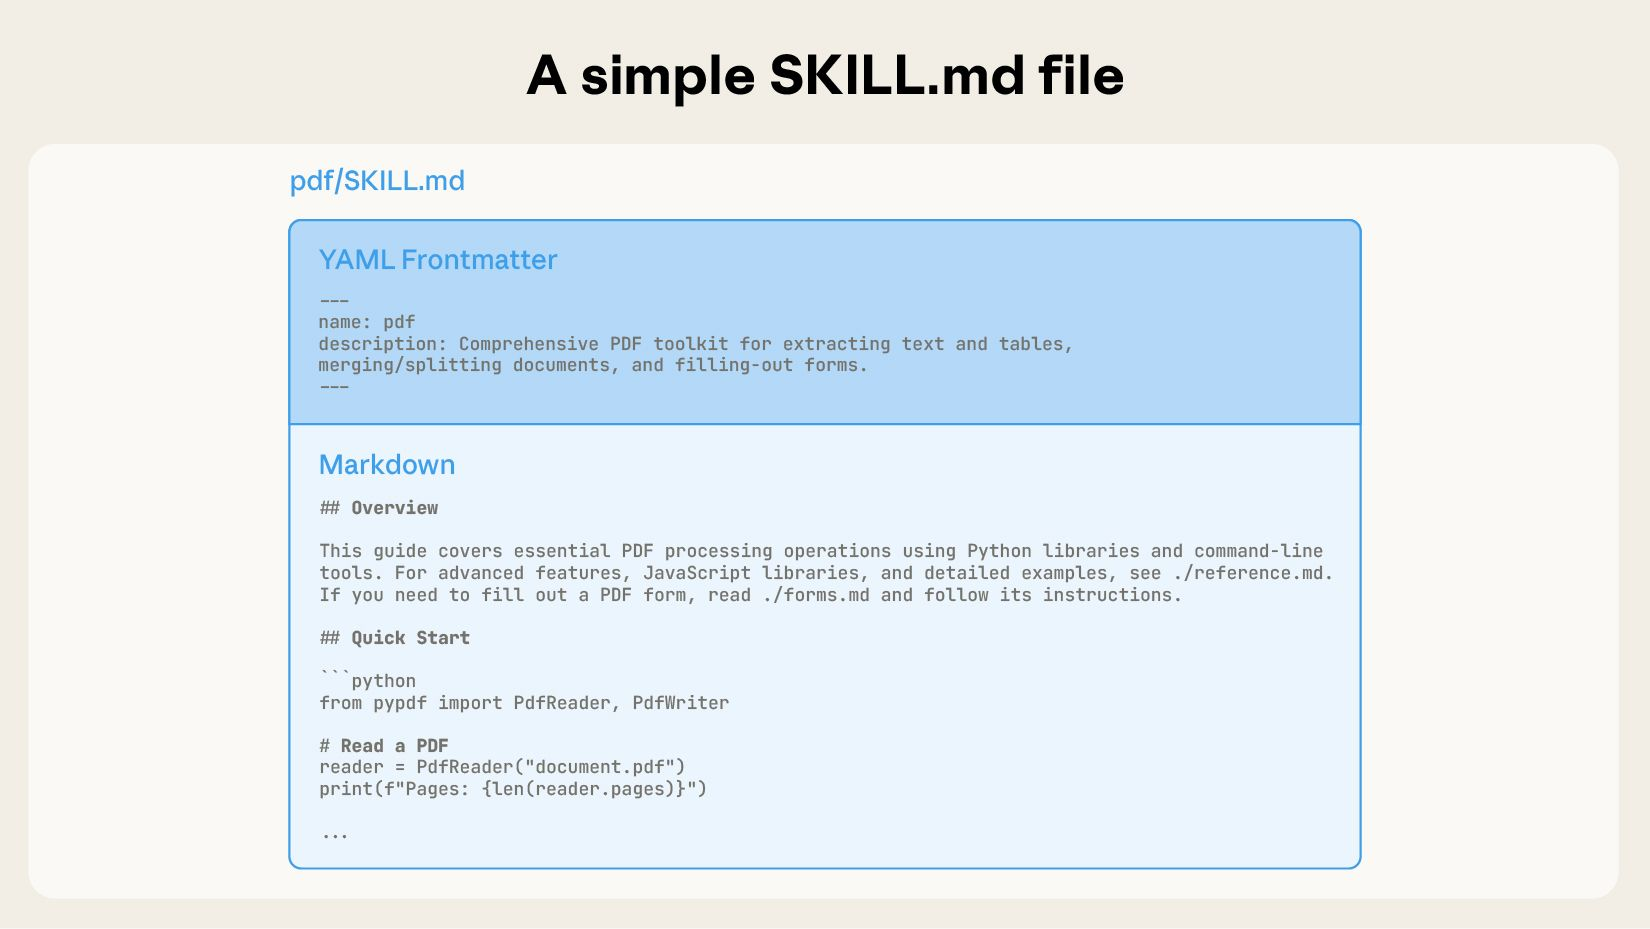
\includegraphics[width=0.92\linewidth]{assets/agent-skills-equipping-agents-skill-metadata.jpg}
\end{center}

\textbf{“Skills 真的这么有用吗？”}这是我最初读相关文章时反复问自己的问题，毕竟它的设计实在太简单。但现在，我绝大部分任务都有项目级和个人级的 Skills 来降低\textbf{控制 / 对齐}成本：让 Agent follow 我设计好的流程，让模型的输出风格和内容对齐我的偏好。从 \weblink{https://www.cs.utexas.edu/~eunsol/courses/data/bitter_lesson.pdf}{The Bitter Lesson} 的长期视角看，把人类知识硬编码进 AI 系统往往不是最可扩展的路线；但在具体的任务工程里，我们要的不是推进通用智能的边界，而是把任务高效做完，把自己的\textbf{思考预算}留给真正需要品味和判断的环节。Skills 的整个定义也很符合 Anthropic 的工程价值观：\textbf{\textit{Do the simple thing that works}}。

Skills 给 Agent 提供的是什么？Anthropic Skills 团队负责人 Barry Zhang 在 \weblink{https://youtu.be/CEvIs9y1uog}{AI Engineer 的 talk} 中的定义是 “\textbf{\textit{composable procedural knowledge for agents}}”。这里的关键词是\textbf{程序性知识（Procedural Knowledge）}。与事实性知识（知道是什么）不同，程序性知识描述的是 怎么做 以及 怎样算做对。它与具体场景绑定，因此也可以理解为从特定领域蒸馏出的实践经验（Domain Expertise）。

\begin{notebox}[为什么叫 Procedural Knowledge 而不是 Workflow Knowledge 呢？]
我最早写这篇博客时，凭直觉用的是 Workflow Knowledge。后来想搞清楚 Anthropic 为什么专门要用 Procedural 这个词，去翻了下背景：它来自认知科学，跟 declarative knowledge（“知道什么”）相对，指“知道怎么做”的那一类知识（参见 \weblink{https://en.wikipedia.org/wiki/Procedural_knowledge}{Wikipedia: Procedural knowledge}）。

看完我也接受了这个用法。不是每个 Skill 都是流程：一个只固定配色和字体的品牌设计 Skill，很难称为 Workflow Knowledge。Procedural 的范围更大，简单的“按规范做”和复杂的“按流程做”都能兼容。本文之后统一用 Procedural Knowledge（程序性知识）。
\end{notebox}

但只到这里，对我而言还有一个困惑没有解开：\textbf{Skills 的本质是什么？}如果只跟着 Anthropic 的官方叙事走，很容易把它解读成“一种 Agent 能力的打包格式”，这篇也会变成多篇 Anthropic 博客的综合解读，那大可不必由我来写（Opus / GPT 可能更适合）。回到第一性原理想这个问题，结合我之前写博客的一些思考，我的理解从两个点出发。

\begin{center}
  \includegraphics[width=0.62\linewidth]{assets/context-type-definition.png}
\end{center}

\textbf{第一，Skills 本质上就是 Context。}技术上你完全可以在 Skills 文件夹里放任何类型的上下文。按我在\weblink{https://keli-wen.github.io/One-Poem-Suffices/one-poem-suffices/context-engineering/}{《Context Engineering，一篇就够了》}里的分类，既可以是指导性上下文，也可以是信息性上下文：事实数据、API 文档、甚至 RAG 索引。所以“提供什么类型的知识”并不是 Skills 最核心的创新，朴素的 Context 文件也可以提供 Procedural Knowledge。

那为什么最佳实践都表明，Procedural Knowledge 特别适合 Skills 这种格式？我的理解是三个原因：（1）它的触发信号是\textbf{任务类型}：模型看到“生成 PDF 报告”就知道该加载 PDF 流程，靠 Skills 的 \code{description} 做文本分类就够了，不需要向量检索。（2）它的内容\textbf{天然有结构}：步骤、工具、引用，可以映射到文件夹层级。（3）它的复用是\textbf{整包、跨会话}的：同一个流程在不同会话、不同人手里都原样适用，每次被取用的都是同一份完整内容，这样打包的 ROI 才够高。举一个反例，常见的 RAG 场景：一份公司内部的产品 FAQ，触发信号是用户提问的语义（更多需要向量检索，而非任务类型分类），内容是扁平的 Q\&A 对，复用的单位是条目而非整包：每次提问只命中其中几条，且次次不同，不存在一个值得整体加载的“流程”。这种 Context 用 RAG 比用 Skill 更合适。

\begin{questionbox}[读到这里可能有一个很直接的问题：\code{scripts/} 是可执行的 tools，怎么能直接说 Skills 就是 Context？]
我的思考是：第一，我在 Context Engineering 篇把上下文分了三类，除了上面这两类，还有一类\textbf{行动性上下文}：工具的定义和用法本身也是 Context，MCP（Model Context Protocol）就是它的标准化协议，\code{scripts/} 可以看成它的本地版。第二，Skill 从头到尾只负责提供 Context，“能跑”是 Harness/Sandbox 给的能力；把同一个 Skill 放进没有执行环境的 Harness，\code{scripts/} 就退化成一段可以阅读的参考代码。下文的 1.3 节会展开解释。
\end{questionbox}

\textbf{第二，Skills 的设计体现了 Push $\to$ Pull 的范式转移。}这个判断源自我在写 \weblink{https://keli-wen.github.io/One-Poem-Suffices/one-poem-suffices/just-in-time-context/}{《Just-in-Time Context，一篇就够了》}时的思考。传统模式下，人类构建检索系统，把自认为模型可能需要的上下文灌进去（Push）；当模型能力越过某个智能阈值，这种\textbf{硬编码}反而成了限制。所以 Anthropic 很早就开始力推 Just-in-Time Context：只给\textbf{引用和目录}，把上下文窗口尽可能留给模型主动的探索（Pull）。Skills 的核心机制，就是 JIT Context 的核心机制：\textbf{引用即上下文（References as Context）}和\textbf{渐进式披露（Progressive Disclosure）}。metadata 常驻 $\to$ body 按需读 $\to$ references 深度探索，正是这个范式的具体实现。

这两点合在一起，才能解释 Skills 为什么长成现在这个样子。所以我的结论会是：\textbf{Agent Skills 是 Just-in-Time Context 的具体实现之一}。后文也会尽量从这两个视角出发，而不是单纯解读官方博客。

基于此，本篇旨在回答三个问题：

\begin{itemize}
  \item \textbf{What？}Skills 作为一种 JIT Context 的实现，具体的格式和机制是什么？它和 Prompt / MCP / Subagent / Memory 等已有机制有什么区别？
  \item \textbf{Why？}为什么是现在，为什么是这种形态？通用 Agent 的崛起和 Skills 之间是什么关系？
  \item \textbf{How？}构建一个好 Skill 的最佳实践是什么？
\end{itemize}

为了保证正文的阅读流畅性，我把一些延伸讨论放进了附录～ 这篇博客“呕心沥血”，写了好几周，希望大家多多支持～

% ---------------------------------------------------------------- Section 1
\section{What is a Skill?}

引言中我先给出了两个观点：Skills 本质是 Context，取用方式是 JIT/Pull。我们先从\textbf{是什么}出发，解释其具体的格式和机制长什么样。

\subsection{格式：一个文件夹}

Anthropic 对 Skill 的定义很简单：

\begin{blockquote}
Skills 是一组组织好的文件，为 Agent 打包可组合的程序性知识。换句话说，它们就是文件夹。这份简单是刻意设计的。\textit{“Skills are organized collections of files that package composable procedural knowledge for agents. In other words, they're folders. This simplicity is deliberate.”}
\end{blockquote}

文件夹可以被人阅读、被 Git 管理、被团队分享，也能被 Agent 用 \code{Read} / \code{Bash} / 文件系统原语操作。任何人都可以在电脑上建一个文件夹，写一个 \code{SKILL.md}，然后所见即所得地迭代。这对于更多的 No-Tech 用户非常友好。

\begin{center}
  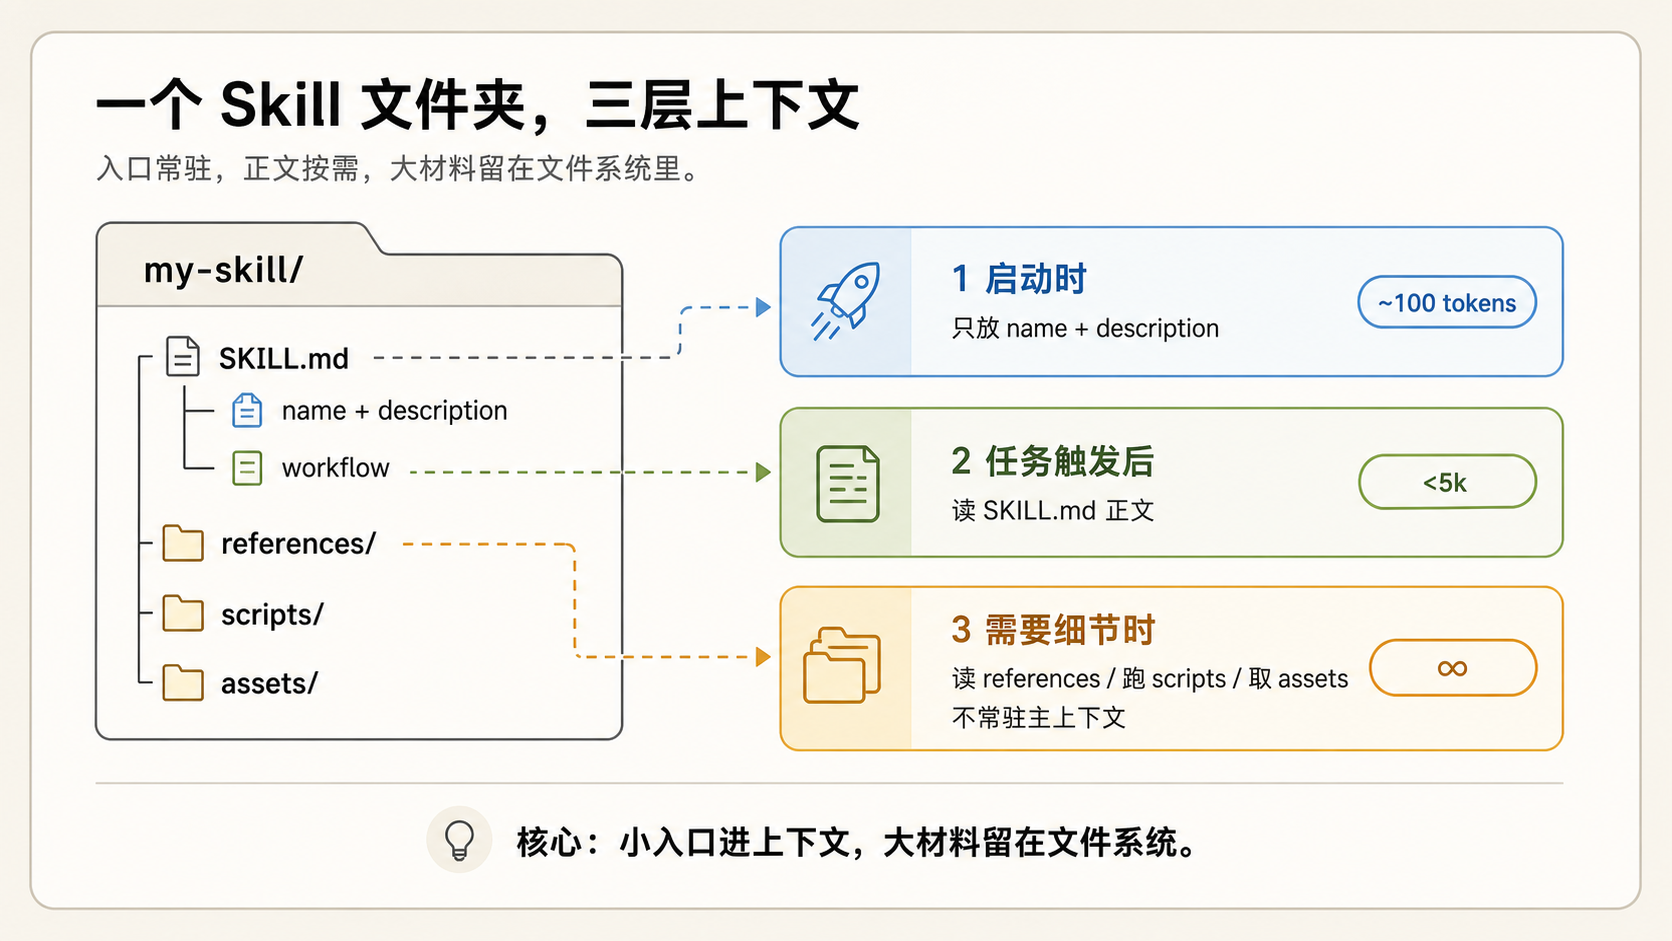
\includegraphics[width=0.94\linewidth]{assets/skill-folder-context-semantics-gpt.png}
\end{center}

这张 GPT 画的图展示了 Skill 核心的结构与设计：\textbf{只有少量 metadata 常驻上下文，作为 trigger 让 Agent 决定要不要进一步加载；其余所有内容都留在文件夹里，由 Agent 按需自行拉取。}三层结构对应的 token 量级：

\begin{itemize}
  \item \textbf{第一层 metadata}（\code{name} + \code{description}）：约 \textbf{100 token}，启动时预加载进 System Prompt
  \item \textbf{第二层 \code{SKILL.md} 正文}：Anthropic 建议控制在 \textbf{500 lines / 5,000 token 以内}，被触发后才读
  \item \textbf{第三层 bundled files}（\code{references/}、\code{scripts/}、\code{assets/}）：\textbf{无上限}，按路径按需打开
\end{itemize}

\begin{tipbox}
我与一些朋友交流时发现，很多人不知道 Skills 的 metadata 会常驻 System Prompt，就像不知道 MCP 也会把 Tools 的定义注入上下文。如果忽略概念的包装，把两者都理解成 Context，那它们出现在上下文窗口里就是自然的事。

也因此，Skills 并不是越多越好。Anthropic 给的参考线是：同时启用的 Skills 到了 20-50 个，就该重新评估和取舍；常见的做法是合并同类 Skill，把具体内容下放到 \code{references/}，交给渐进式披露。或者走 \weblink{https://platform.claude.com/docs/en/agents-and-tools/tool-use/tool-search-tool}{Tool Search Tool 的范式}。
\end{tipbox}

\subsection{Skills 的核心机制}

Skills 的核心机制和 JIT Context 一致：\textbf{引用即上下文 + 渐进式披露}。这里重述下 JIT 博客中的一些结论：理解这套机制有一个前提：\textbf{上下文是边际效益递减的有限资源}。上下文窗口里的 token 越多，模型从中提取准确信息的能力越弱（\weblink{https://research.trychroma.com/context-rot}{context rot}），而 Agent 架构天然比普通对话消耗更多 token（Anthropic 的数据是 \weblink{https://www.anthropic.com/engineering/multi-agent-research-system}{4 倍以上}）。所以\textbf{管理好上下文窗口，就是在管理 Agent 的推理质量}。

\weblink{https://platform.claude.com/docs/en/agents-and-tools/agent-skills/best-practices}{Agent Skills Best Practices} 里有一句话：\textbf{“The context window is a public good.”}上下文窗口要同时容纳 System Prompt、对话历史、工具结果、其他 Skill metadata 和当前任务材料。Skill 的三层结构就是在管理这份公共资源：第一层 metadata 做触发判断（这个任务需不需要我？），第二层 body 给流程和指令（具体该怎么做？），第三层 \code{references/} / \code{scripts/} 提供细节和执行力（遇到具体问题去哪查、用什么工具？）。Agent 逐层深入，每一层只在需要时才加载，不浪费注意力预算。

\subsection{为什么 Skills 需要 scripts/？}

\code{scripts/} 是 Skill 可选的组件。大多数 Skill 一开始\textbf{不需要}它（也没有它），只写 \code{SKILL.md} 和 \code{references/} 已经够用。\code{scripts/} 是 Skill 的\textbf{上限}，不是入门门槛。

\textbf{什么时候该把写给模型看的指令，换成给模型跑的脚本？}很简单：\textbf{当某个动作和语义理解无关、需要 100\% 可复现时。}Anthropic 举过一个例子：Claude 总在幻灯片任务里反复写同一段 styling Python，后来他们让 Claude 把它保存进 Skill，作为给未来自己的工具。\textbf{重复、稳定、可验证的动作，就该从语言解释变成可执行的 script。}

\code{scripts/} 本质上就是 Tools（Anthropic 的原话也是 “scripts as tools”）。而工具对模型来说一直都是 Context：模型并不真的“执行”任何东西，它看到工具的定义（绝大部分 Harness 在创建新 Session 时会把工具定义注入上下文），吐出一行调用，再等结果以 token 回来，执行发生在模型之外的 Harness 里。所以引言说“Skills 本质是 Context”是把 \code{scripts/} 算在内的：它就是行动性上下文，只是定义放进了文件系统。这带来两个传统 Tools 没有的性质。其一，\textbf{定义可读可改}：传统 Tool 的描述（docstring）写得再含糊，模型也只能将就着用；script 是文件，代码本身就是最准确的定义，模型必要时可以直接读源码并做改动，不用时则安静地待在文件系统里。其二，\textbf{它不承诺可执行}：script 只提供“这里有个工具、这么用”的上下文，真跑起来缺依赖、环境不对，都要 Agent 自己当场解决（\weblink{https://agentskills.io/specification\#frontmatter}{frontmatter} 的 \code{compatibility} 字段就是用来提前声明环境要求的）。

\opfig[0.94]{assets/equipping-agents-skill-file-structure.jpg}{Skill 的 metadata 挂在 agent 配置中，文件夹内容则活在 agent 虚拟机的文件系统里，与 Bash / Python / Node 运行时为邻；MCP server 在远端。Source: \weblink{https://www.anthropic.com/engineering/equipping-agents-for-the-real-world-with-agent-skills}{Equipping agents for the real world with Agent Skills}}

第二个收益是\textbf{省 token}。当 Agent 读一个 reference，是把内容按需拉进上下文窗口；而跑一个 script，效果上和派一个 Subagent 类似（把 Subagent 理解成一个 Agentic Tool 即可），起到了\textbf{上下文隔离}的作用。脚本本体、它处理的数据、中间过程，全都隔离在“珍贵的主上下文窗口”外，窗口里只剩一行调用和一行结果（当然有时候可能有很多日志信息）。举个不恰当的例子：让模型用 generation tokens 一行一行吐出 1MB CSV 的排序结果，既慢又贵；一行 \code{sort} 就够了。如果说渐进式披露对注意力预算的控制是“按需读取”，\code{scripts/} 就是更进一步的“根本不用读”：把复杂、耗 token 的流程直接 tool 化，省掉不必要的注意力消耗。

\textbf{\code{scripts/} 和 MCP 有什么区别？}

两者都是行动性上下文，但分工不同。MCP 解决\textbf{连接}：把外部系统（数据库、SaaS、内部服务）用标准协议接进来，工具由 server 托管，连上了就能用。\code{scripts/} 解决\textbf{流程内的确定性}：它从属于 Skill 所描述的那套流程，把其中重复、脆弱、和语义理解无关的环节固化成代码，换来稳定性和 token 效率；它通常不连接任何外部系统，就在本地跑，跑不起来也没有人兜底，要 Agent 自己修环境。所以常见的组合是 \textbf{MCP 拿数据 $\to$ \code{scripts/} 清洗渲染 $\to$ 模型基于 Skill 的领域知识判断总结}：连接交给协议，确定性交给脚本，判断留给模型。详见 \weblink{https://claude.com/blog/extending-claude-capabilities-with-skills-mcp-servers}{Extending Claude with Skills and MCP}。

另外，\code{scripts/} 也是 Skill 对部署唯一提出要求的部分：纯 Context 的 Skill，任何能读文件的 Agent 都能用；带上脚本，就需要一个干净的 Sandbox。在涉及部署时需要做 Agent Framework 两种流派的取舍，具体内容见 Appendix B。

\subsection{如何为 Skills 分类？}

既然 Skills 本质是 Context，那分类也可以从 Context 的视角来看。一个 Skill 文件夹里其实混合了三种上下文（对应 \weblink{https://keli-wen.github.io/One-Poem-Suffices/one-poem-suffices/context-engineering/}{Context Engineering 篇的上下文三分类}）：

\begin{itemize}
  \item \textbf{指导性上下文}：\code{SKILL.md} 里的流程规范、质量标准、判断原则，告诉模型“该怎么做”
  \item \textbf{信息性上下文}：\code{references/} 里的参考资料、模板、数据，告诉模型“需要知道什么”
  \item \textbf{行动性上下文}：\code{scripts/} 里的可执行代码，告诉模型“可以跑什么”
\end{itemize}

这个对应关系只是典型印象，不是硬性规定。\code{references/} 里完全可以放一份风格规范（指导性），\code{SKILL.md} 里也少不了背景信息（信息性）。这里主要侧重说明的是 Skills 可以包括各类上下文。不同 Skill 侧重不同。一个品牌设计 Skill 可能只有指导性上下文（配色规范、字体要求）；一个 PDF Skill 三类都有（流程 + 参考文档 + Python 脚本）。

Anthropic 还提供了另一个互补的分类视角，从\textbf{行为目的}和\textbf{知识来源}两个维度来看（来自 \weblink{https://claude.com/blog/improving-skill-creator-test-measure-and-refine-agent-skills}{Improving skill-creator} 和 \weblink{https://youtu.be/CEvIs9y1uog}{AI Engineer talk}）：

\begin{itemize}
  \item \textbf{行为目的}：区分 Skills 是在\textbf{补模型做不稳的能力}（Capability Uplift，例如 PDF 解析、Office 文档处理），还是在\textbf{固化流程和偏好}（Encoded Preference，例如 PR Review checklist、周报格式、commit message 约定）。
  \item \textbf{知识来源}：区分 Skills 是\textbf{平台方提供的通用能力}（Anthropic 官方的 \code{pdf} / \code{docx} 等 Skill），\textbf{第三方产品的最佳实践}（Vercel / Supabase 等把自家 API 用法封装成 Skill），还是\textbf{你自己 / 团队 / 组织的工作方式}（Coding Harness 偏好、团队 PR 模板、内部审查流程）。
\end{itemize}

个人觉得“行为目的”这个分类视角挺好，目前对我效率提升最高的，仍是固化流程和偏好这一类 Skills。

% ---------------------------------------------------------------- Section 2
\section{Skill vs Prompt / MCP / Subagent / Memory}

把 Skills 和相关概念放在一起比较，区别其实很清晰：它们要么是不同类型的 Context，要么是不同的取用方式。Anthropic 在 \weblink{https://claude.com/blog/skills-explained}{Skills Explained} 里给过一张完整的对比表格，下面我从自己的视角补充一些理解。

\subsection{vs Prompt / CLAUDE.md / AGENTS.md}

Prompt、\code{CLAUDE.md}、\code{AGENTS.md} 和 Skill 都在告诉 Agent “怎么做”（更偏指导性上下文），区别主要在\textbf{什么时候加载}：

\begin{optable}
\begin{tabularx}{\linewidth}{@{}ll>{\raggedright\arraybackslash}X@{}}
\toprule
\tabhead{机制} & \tabhead{加载时机} & \tabhead{典型场景} \\
\midrule
Prompt & 当前对话内输入 & 一次性请求、临场修正 \\
\code{CLAUDE.md} / \code{AGENTS.md} & 进入项目即全量加载 & 项目结构、测试命令、代码风格、禁止事项 \\
Skill & 任务语义命中才加载 & 发布检查、数据库 migration、按公司格式生成评审文档 \\
\bottomrule
\end{tabularx}
\end{optable}

\begin{blockquote}
如果你发现自己在不同对话里反复输入同一段 Prompt，那就把它做成一个 Skill。\textit{“If you find yourself typing the same prompt repeatedly across conversations, create a Skill instead.”}
\end{blockquote}

如果你发现在完成一类任务时需要输入同一段指令 5 次以上，那这段指令就应该被持久化为\textbf{知识}。但有进一步的问题需要思考：\textbf{到底是写成 Skill，还是更新到 \code{CLAUDE.md}？}

区别在这段 Context 的\textbf{作用域}。\code{CLAUDE.md} 是项目级的，每次对话都全量常驻 System Prompt，适合放“永远成立”的规则（项目结构、测试命令、代码风格）。而反复出现的指令往往只在\textbf{某一类任务}里才需要，这种任务级的知识写成 Skill，让它语义命中才加载，不占无关对话的注意力预算。

如果用 Push / Pull 的范式进行解释：Prompt 和 \code{CLAUDE.md} 都是 \textbf{Push}（人类主动塞进去），Skill 是 \textbf{Pull}（Agent 判断需要时才加载）。三者不互斥，按加载时机自然分层。

\subsection{vs MCP}

“MCP 和 Skill 有什么区别？”“有了 Skill 是不是就不需要 MCP 了？”这两个问题我见过很多次，但它们本身就问偏了：两者是兼容且互补的，都在扩展 Agent，只是扩展的方向不同。

Anthropic 的 \weblink{https://claude.com/blog/extending-claude-capabilities-with-skills-mcp-servers}{Extending Claude with Skills and MCP} 博客里有一个厨房类比：\textbf{MCP 像一间装备齐全的厨房}，灶台、刀具、食材、冷柜，对应外部系统、数据库、文件、业务 API；\textbf{Skill 像一份菜谱}，告诉你先做什么、火候多少、什么时候下料。\textbf{模型}则是站在中间的厨师：厨房给它原料和工具，菜谱给它流程，它负责判断和临场发挥。

两者的关系可以表述为：\textbf{“MCP provides connectivity; skills provide expertise.”}前者解决“能不能拿到”，后者解决“知不知道怎么用”。例如你想让 AI 帮你投资：MCP 让 Agent 接入你的账户，获取持仓信息、执行交易操作；Skills 负责指导决策流程，例如给你的 Agent 接入一个巴菲特 Skill。

而且两者是\textbf{多对多}的关系：一个财务分析 Skill 可以同时编排好几个数据源 MCP（行情一个、财报一个、研报一个），一个 GitHub MCP 也可以被 Code Review、Issue 分类、Release 等多个 Skill 复用。两个生态互相增强，而非互相替代。

\begin{center}
  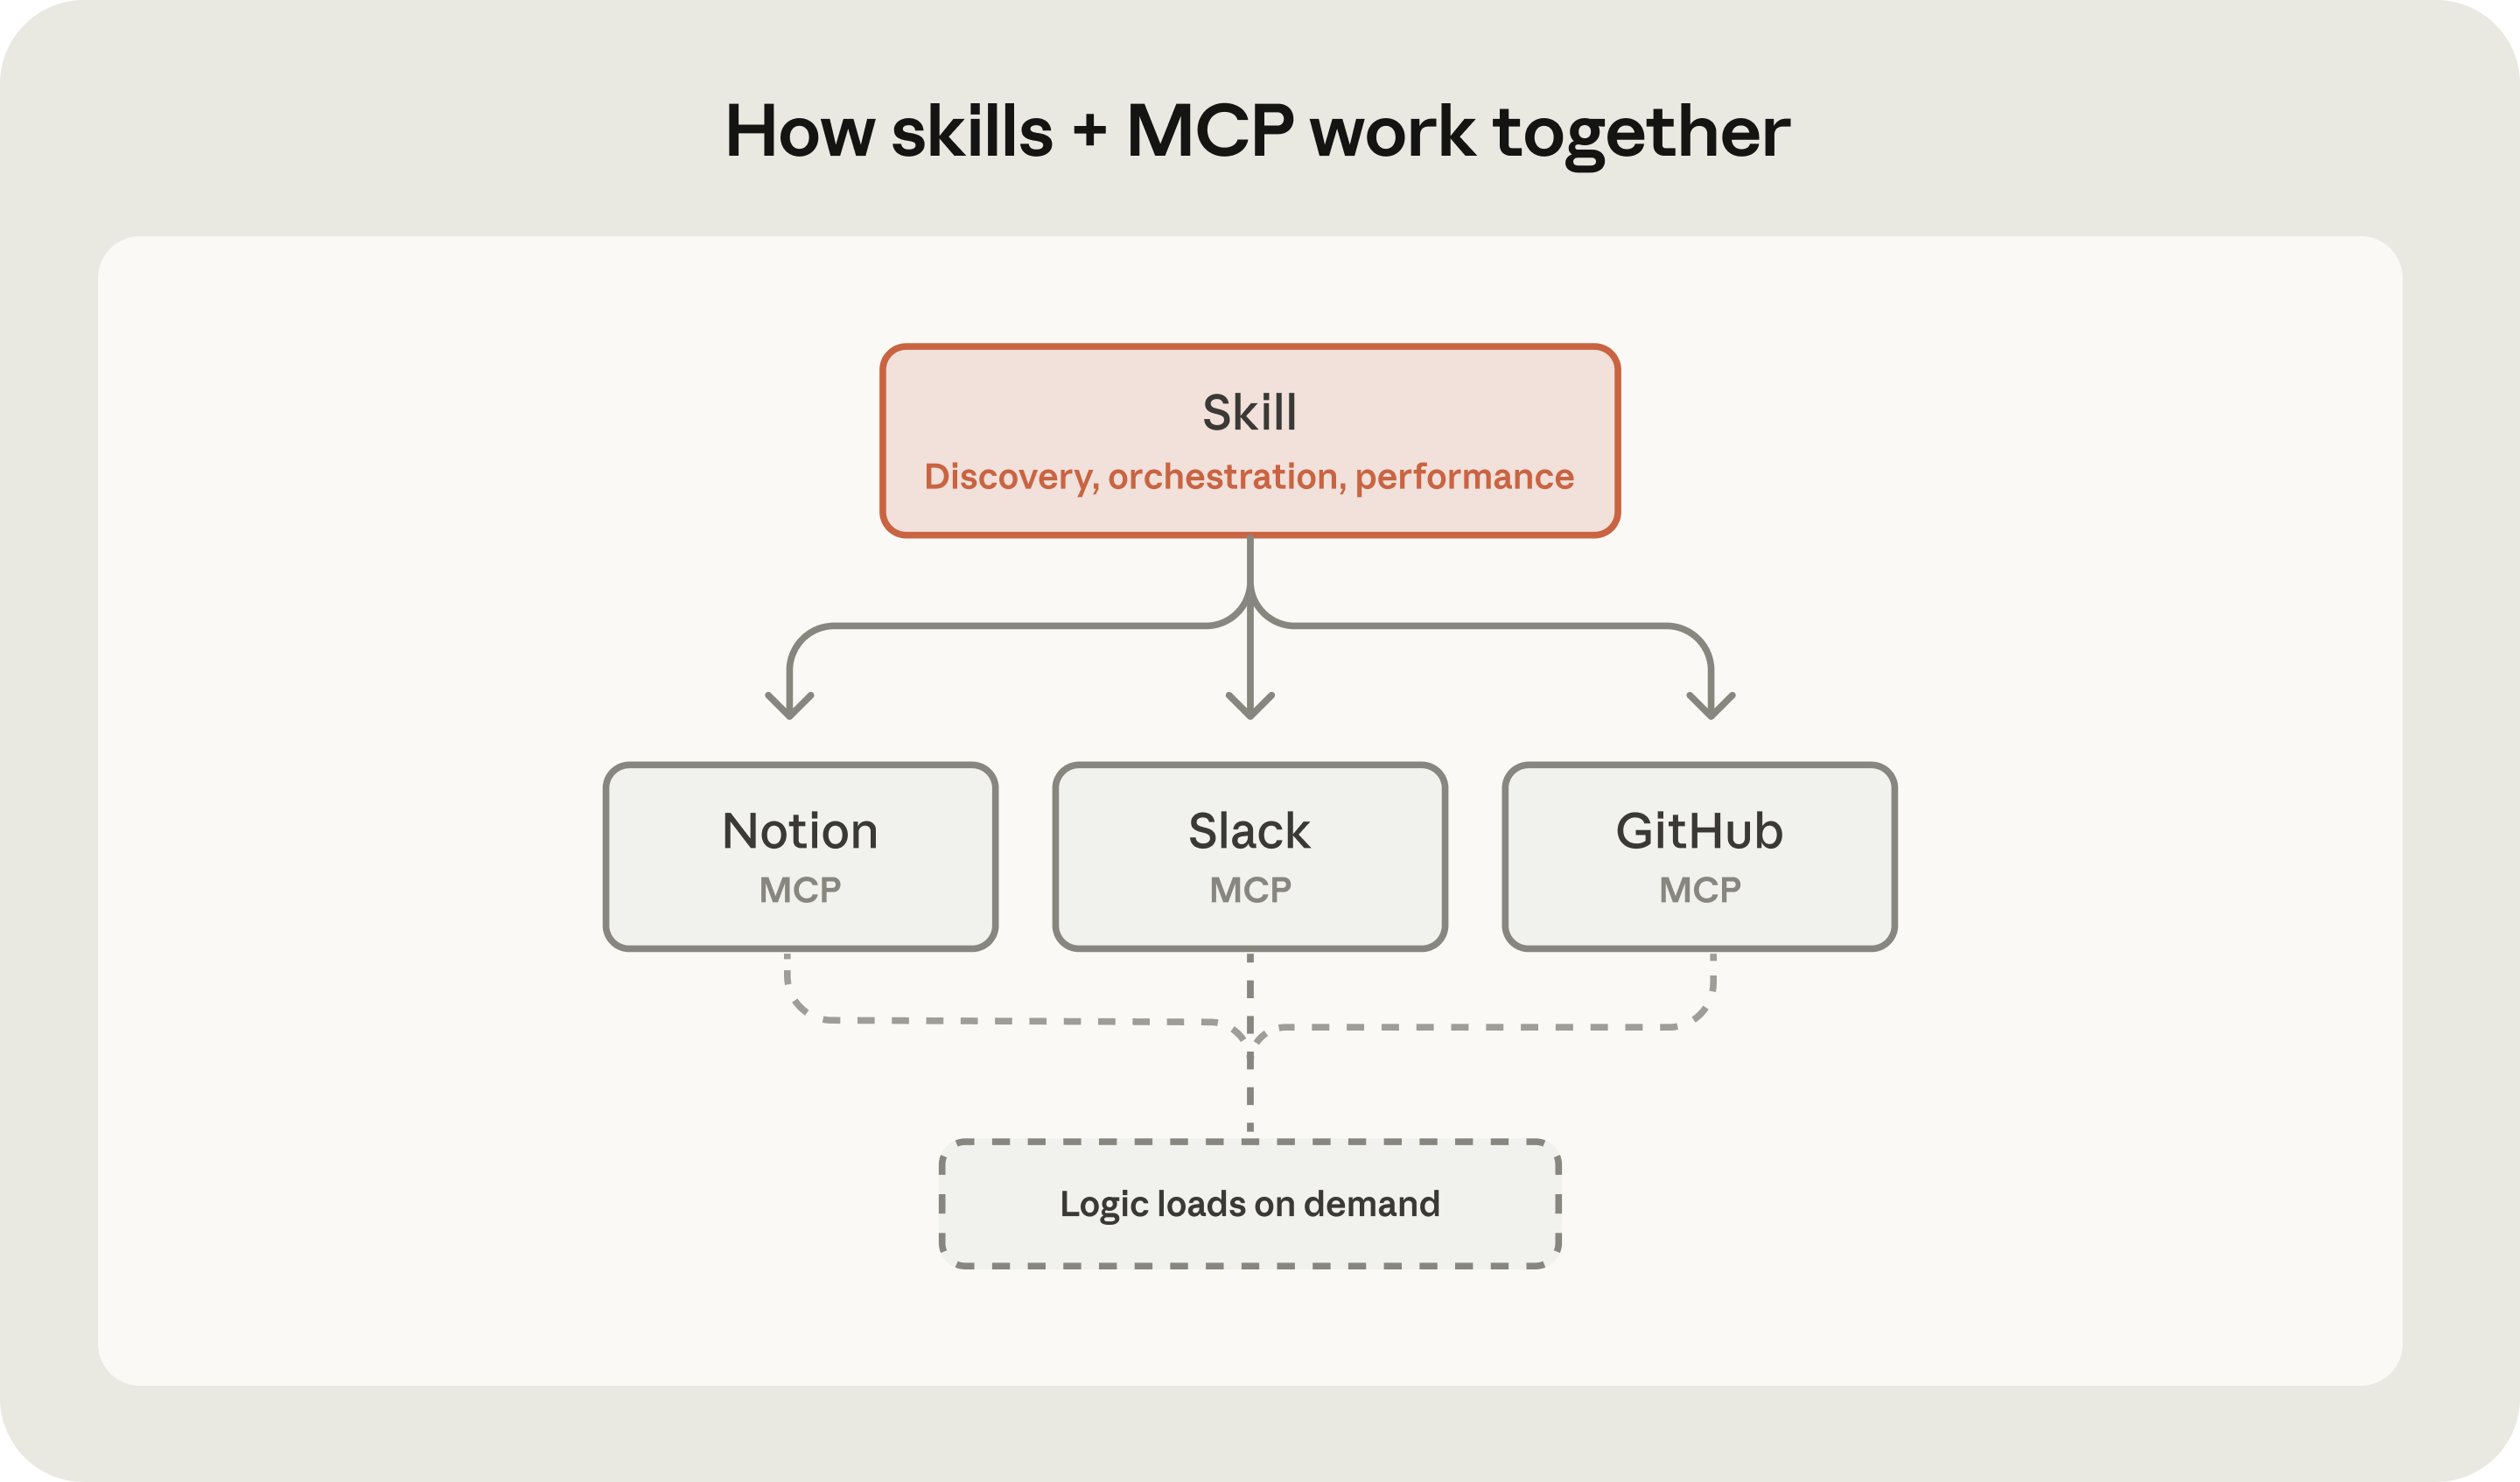
\includegraphics[width=0.8\linewidth]{assets/agent-skills-skills-mcp-skills-mcp-diagram.png}
\end{center}

从 Context 的角度看：MCP 提供的基本全是\textbf{行动性上下文}：工具定义、工具结果，加上把外部数据搬进窗口的通道（严格说 MCP 规范里还有 \code{prompts} 和 \code{resources} 两类原语，但生态的重心在 \code{tools}，这里按主流用法讨论）。Skill 文件夹里装载三类上下文（见 1.4 节），但它的重心是\textbf{指导性上下文}：“拿到数据之后该怎么处理”，两者之中只有 Skill 在负责这件事。所以可以说：MCP 决定 Agent 能调用什么，Skill 决定它知道怎么用。两者不在同一层，是互补的。

\subsection{vs Subagent}

Subagent 和 Skill 其实不在一个层面上，不太能直接比较。Subagent 是一种\textbf{架构机制}：它有独立的 Context Window、独立的工具权限，主 Agent 把一块任务连同 Handoff 上下文交给它，只取回最后结论。它有很多效果，包括改变复杂任务执行的拓扑结构，实现更高级的智能体系统编排；scaling 更多 tokens 做子任务的 verification；以及上下文隔离，把复杂信息流隔离出去，别污染主上下文（\weblink{https://keli-wen.github.io/One-Poem-Suffices/one-poem-suffices/context-engineering/}{Context Engineering，一篇就够了}中的 \textbf{Isolate}）。而 Skill 是一层\textbf{可复用的专业知识}，它本身不负责隔离任务流，只负责“这件事该怎么做”。

那它们怎么联系起来？我个人觉得关键在编排 Subagent 时的一个必要环节：\textbf{每次派生 Subagent，都要给它足够的 Handoff 上下文}，包括任务背景、工具用法和流程规范。当你的 Agent 反复为\textbf{同类任务}派生 Subagent 时，这些上下文在不同 delegation 之间高度重复，同一套东西一遍遍重讲。（例如我之前每次 spawn 新的 Subagent 时，都需要显式要求它基于任务类型按我的规范做进度记录，特别麻烦）

\begin{center}
  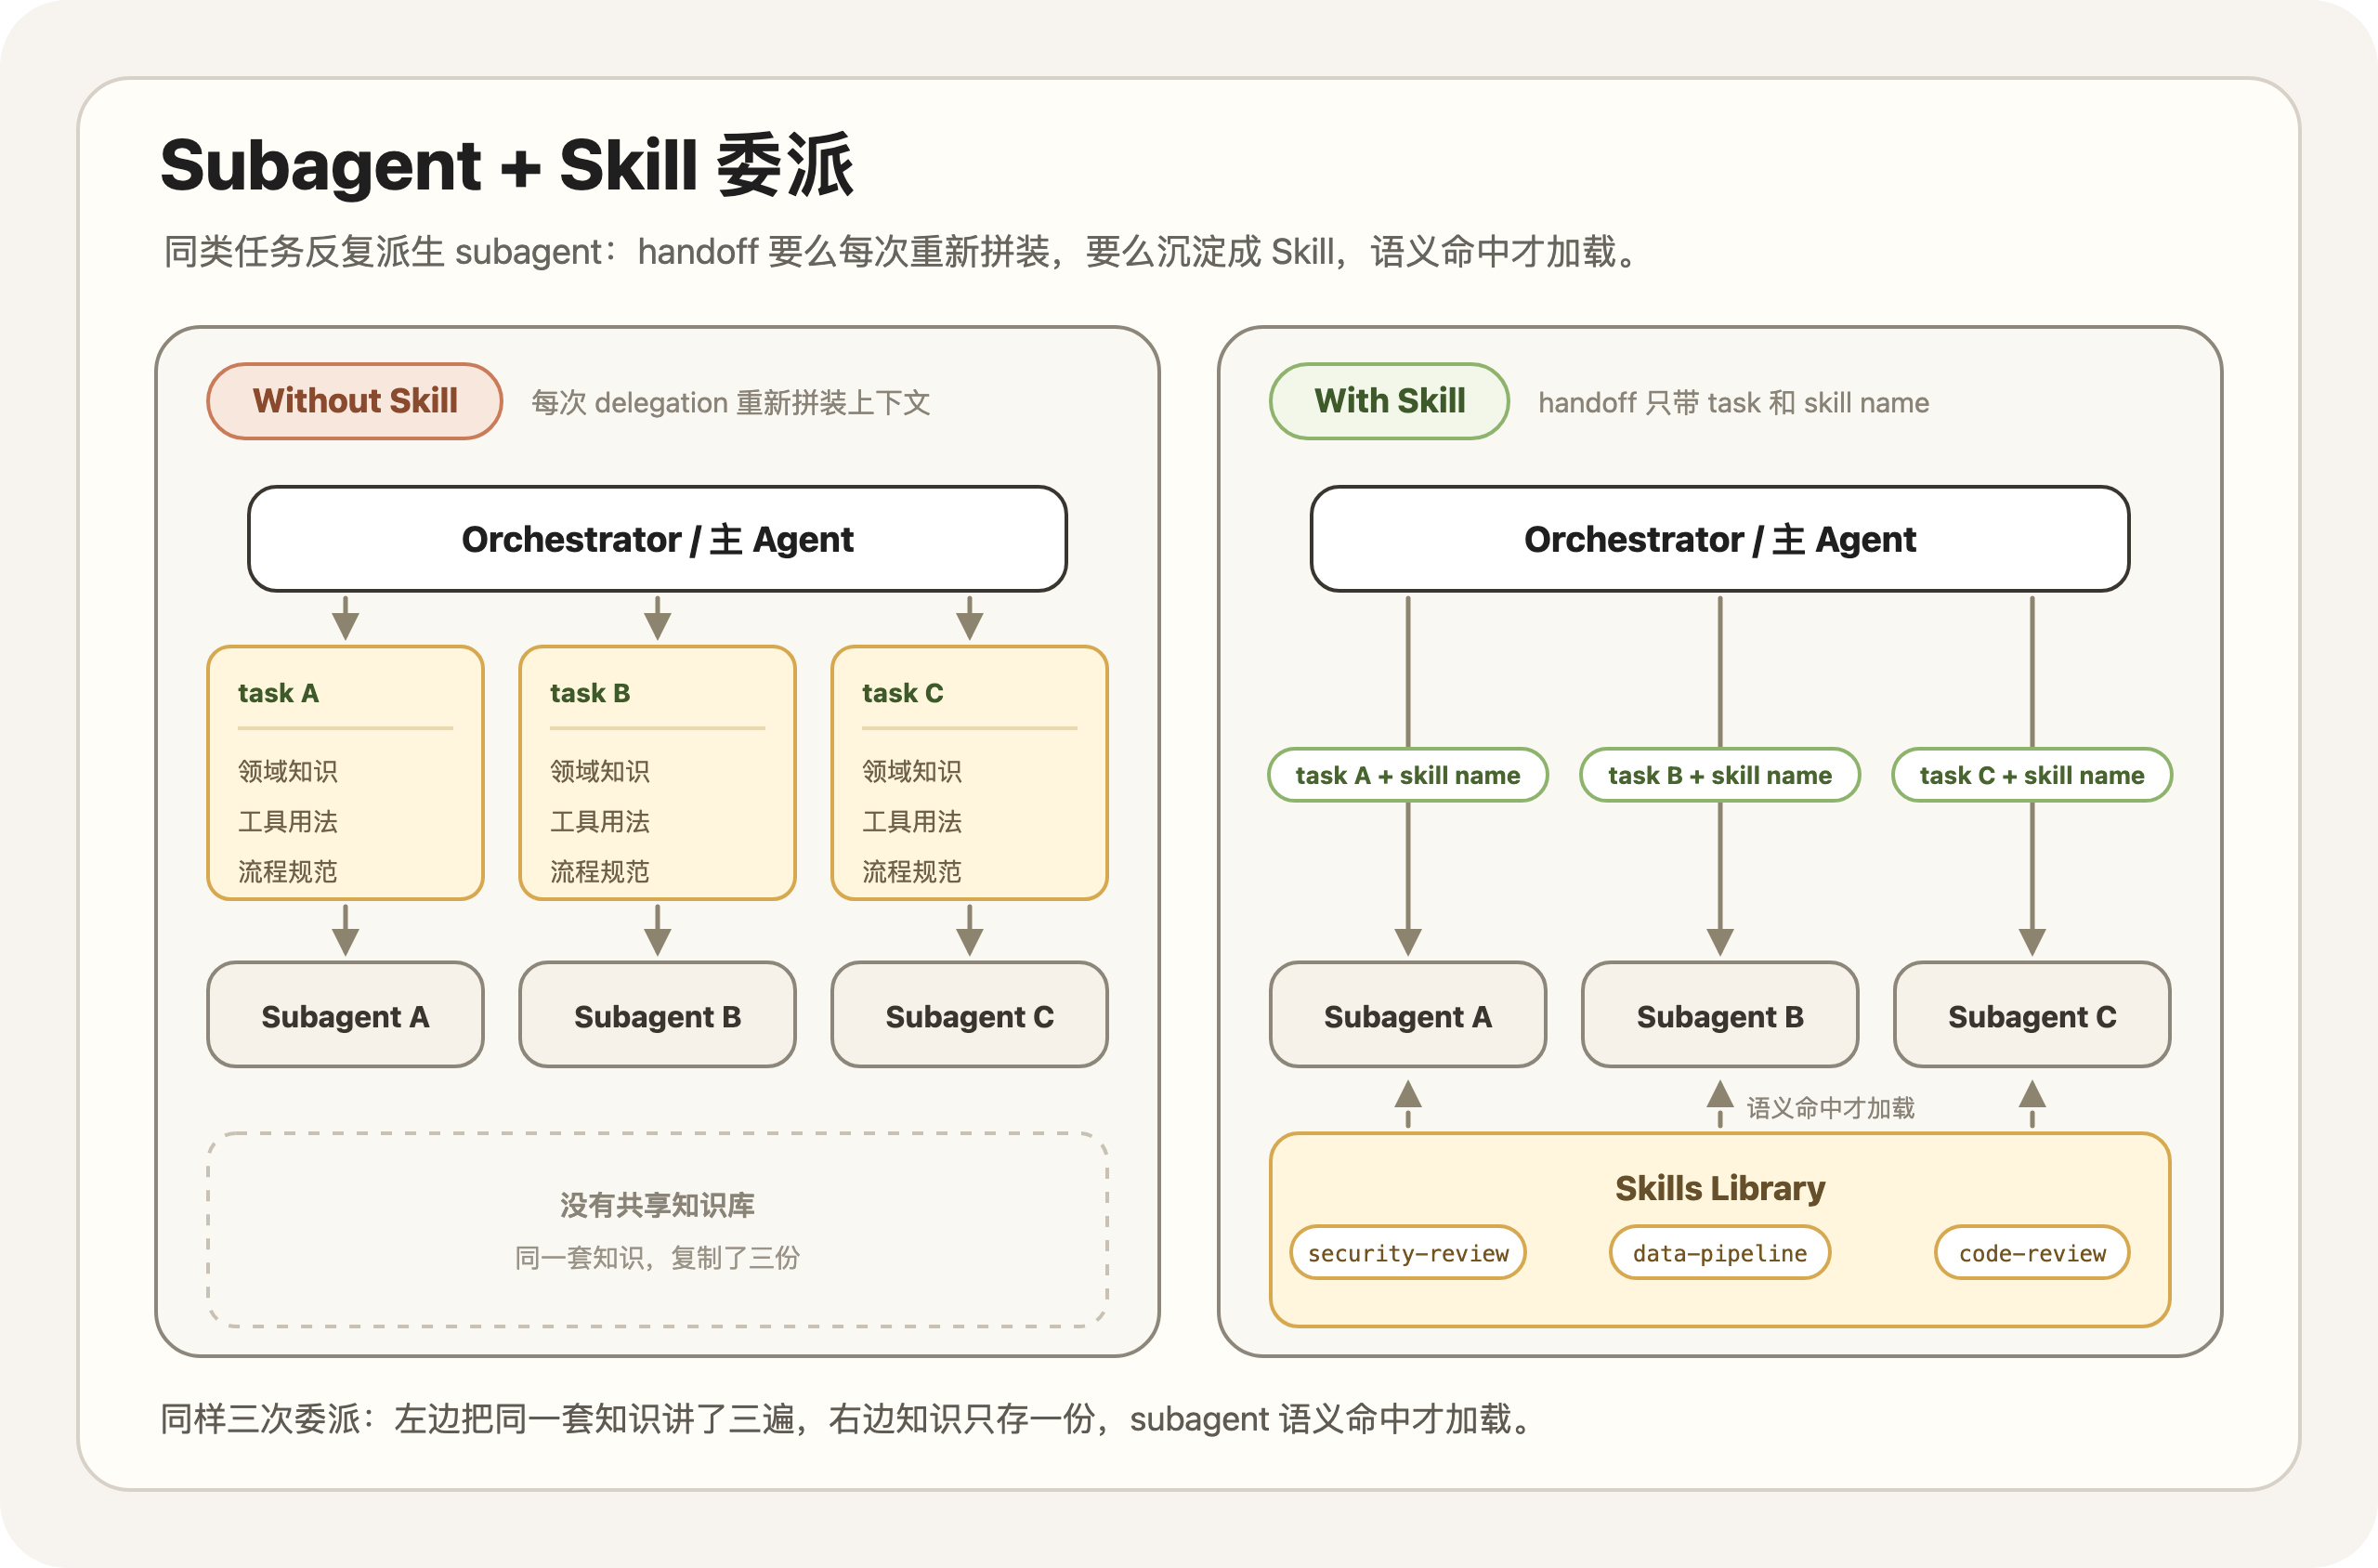
\includegraphics[width=0.9\linewidth]{assets/subagent-delegation-with-skill_claude.png}
\end{center}

Skill 正好补上这一环。把这套重复的上下文和工具用法沉淀成一个 Skill，Subagent 派生时不必每次重新拼装，语义命中就加载。Anthropic 也在博客中推荐了 Subagent 和 Skills 的组合。例如，在我自己的项目中，如果是数据库实现任务，Orchestrator Agent 会基于我的 \code{my-work} Skill（为了方便理解，这里改了下名字）设计 verify checklist，要求另一个 Agent 最后用 \weblink{https://github.com/supabase/agent-skills/tree/main/skills/supabase-postgres-best-practices}{supabase-postgres-best-practices Skill} 做 Review。如果是前端相关任务，则会自动要求用 \weblink{https://github.com/vercel-labs/agent-skills/blob/main/skills/react-best-practices/SKILL.md}{react-best-practices Skill} 做 Review。整个流程很自然，也可以进一步配合 Hooks。

\begin{blockquote}
在 Claude Code 和 Agent SDK 中，Subagent 可以访问并使用 Skills：让专精分工的 Subagent 带上可携带的专业知识，是非常强的组合。\textit{“In Claude Code and the Agent SDK, subagents can access and use Skills, creating powerful combinations where specialized subagents leverage portable expertise.”}
\end{blockquote}

再举一个更通俗的例子，你让 Agent 帮你做一份竞品分析报告。主 Agent 派一个 Subagent 专门负责数据收集和分析，这个 Subagent 加载 \code{competitive-analysis} Skill（里面定义了分析框架：先看定位、再比功能、再看定价，最后给一页优劣势对比），在隔离窗口里跑完流程，主 Agent 只接收最终的分析结论和关键数据。如果切换为 Deep Research 任务，你只需要去 GitHub 上下载一个 \code{deep-research} Skill 替换 \code{competitive-analysis}。

\textbf{所以我更倾向认为，“Skill 化的 Subagent”会是更自然的编排范式}：Subagent 提供隔离的执行环境，Skill 提供可复用的专业流程，编排时不再靠 Agent 基于 Session 构建一堆重复 Context，而是让 Subagent 按需加载该用的 Skill。（有点像现代公司里的交接模式～ 当然，向人类组织对齐未必就是 Agent 的最佳实践）

\subsection{vs Memory}

还有一个值得思考的对比，Memory 也是跨会话的，它和 Skill 是什么关系？基于 Context 的视角，两者都是跨会话持久化的 Context，没有本质区别。Memory 系统基于不同的提取偏好（事实或者流程知识）可以得到不同类型的 Memory Context。这里我以 Claude Code 中的 Memory 实现为例：\textbf{Memory 是 Agent 自动更新的、关于你和你的项目的零散事实与偏好；Skill 则是人主导更新的、关于某类任务该怎么做的程序性知识。}这个定义可能在之后不完全准确。下面结合社区整理的非官方 Claude Code 源码镜像，把我观察到的几点写下来。

\begin{infobox}[可跳过的深水区]
接下来几段是基于“非官方”源码、对 Claude Code Memory 读写机制的拆解。如果你只关心 Memory 和 Skills 的差异结论，可以直接跳到下方\textbf{差异主要在三个地方}，不影响后续阅读。就当是一次渐进式披露：这里是 reference file。
\end{infobox}

在读取方式上，Memory 和 Skills 都是按需读取那套。我基于 Claude Code auto-memory 的机制制作了如下图片。其中上半部分是 Memory 的更新，下半部分则是读取。

\opfig[0.94]{assets/memory-mechanism-loop_claude-v2.png}{Claude Code 中的 auto-memory 机制}

Memory 的写入 Pipeline 是全自动的。如果当前是主会话且开启了 Memory，后台会根据阈值设置（默认每轮对话后）Fork 一个继承主模型的 Subagent（继承是为了共享 Prompt Cache）。Subagent 会被要求重点分析最近一轮的对话，并与已有记忆进行\textbf{比对}：\textbf{如果发现有价值的持久化信号，它会通过新建、修改覆盖（Upsert）或删除已有文件的方式更新 \code{memory/} 目录及 \code{MEMORY.md} 索引}。注意，这里的比对和 Skills 的加载以及下文中的 Memory 加载范式是一样的，Subagent 会先扫描所有记忆条目的 header（名字和描述）确认是要更新还是新建，如果需要更新则会继续读取该记忆条目的完整内容。

读取 Pipeline 也是常驻后台的（当开启了相关 feature）：每当有用户的对话 Request 到来时，一个旁路小模型（代码里是获取 sonnet 但限制 256 tokens 的输出）读取所有\textbf{未被读取}的 Memory 文件的 Header（和 Skills 一样，每条记忆的名字 + 描述），从中挑出至多 5 条，将完整内容拼接为 Memory Context，在推理开始前注入当轮对话。

其中 \code{MEMORY.md} 是类似 \code{CLAUDE.md} 的记忆索引，可以理解为整个记忆库的目录。在 Memory 的读写 pipeline 中它都提供索引作用（符合 Just-in-Time 的原则）。\code{MEMORY.md} 是常驻上下文的。因此，\textbf{它同样服务于主 Agent，当 Memory 读取 pipeline 没有正确的匹配到可能需要的记忆时，主 Agent 可以直接基于 \code{MEMORY.md} 使用 tool call 把希望阅读的记忆读取到上下文中}。

对比两者，Skills 的 metadata 层和 Memory 文件的 header 格式基本一致，\code{SKILL.md} 的主体则对应每个 Memory 文件的具体内容。

那差异主要在三个地方：

\begin{itemize}
  \item \textbf{Context 的类型}：Claude Code 把 Memory 限定为四类（user / feedback / project / reference），基本都是信息和偏好（信息性上下文），源码注释还专门要求只存无法从项目状态推导的东西；Skills 装的更多是程序性知识（指导性上下文）。
  \item \textbf{构建/加载机制}：Memory 的构建由后台 Subagent 周期性“无监督”提取，把关的是 Agent 而非人类；Skills 大多由人构造，经过人的审核。至于加载层面，两者都符合 Just-in-Time Context 的加载逻辑，但召回的决策者有差别：Skill 由主模型自己看 \code{description} 决定加载，Memory 的加载则通常发生在主上下文之外，由旁路模型代为决策。
  \item \textbf{作用域}：Memory 存储项目相关的信息性上下文，通常和项目强绑定。Skills 中的 Context 则更偏向可分享，可迁移。
\end{itemize}

但我个人觉得，如果从 Context 的角度，它们两者区分的边界可以很模糊。一条“提交代码前先跑代码格式检查”的 feedback memory，和 Skill 里的一条规则可以一模一样，只是从加载与更新机制的角度它们会有更多区别。就我个人而言，我的 \code{autoMemoryEnabled} 至今是 false：自动生成、无人筛选的记忆会浪费 tokens，偶尔还对解决问题有副作用。关于 Memory 与 Skills 在持续学习领域的思考放在 Appendix C 中。

\subsection{小结}

\begin{center}
  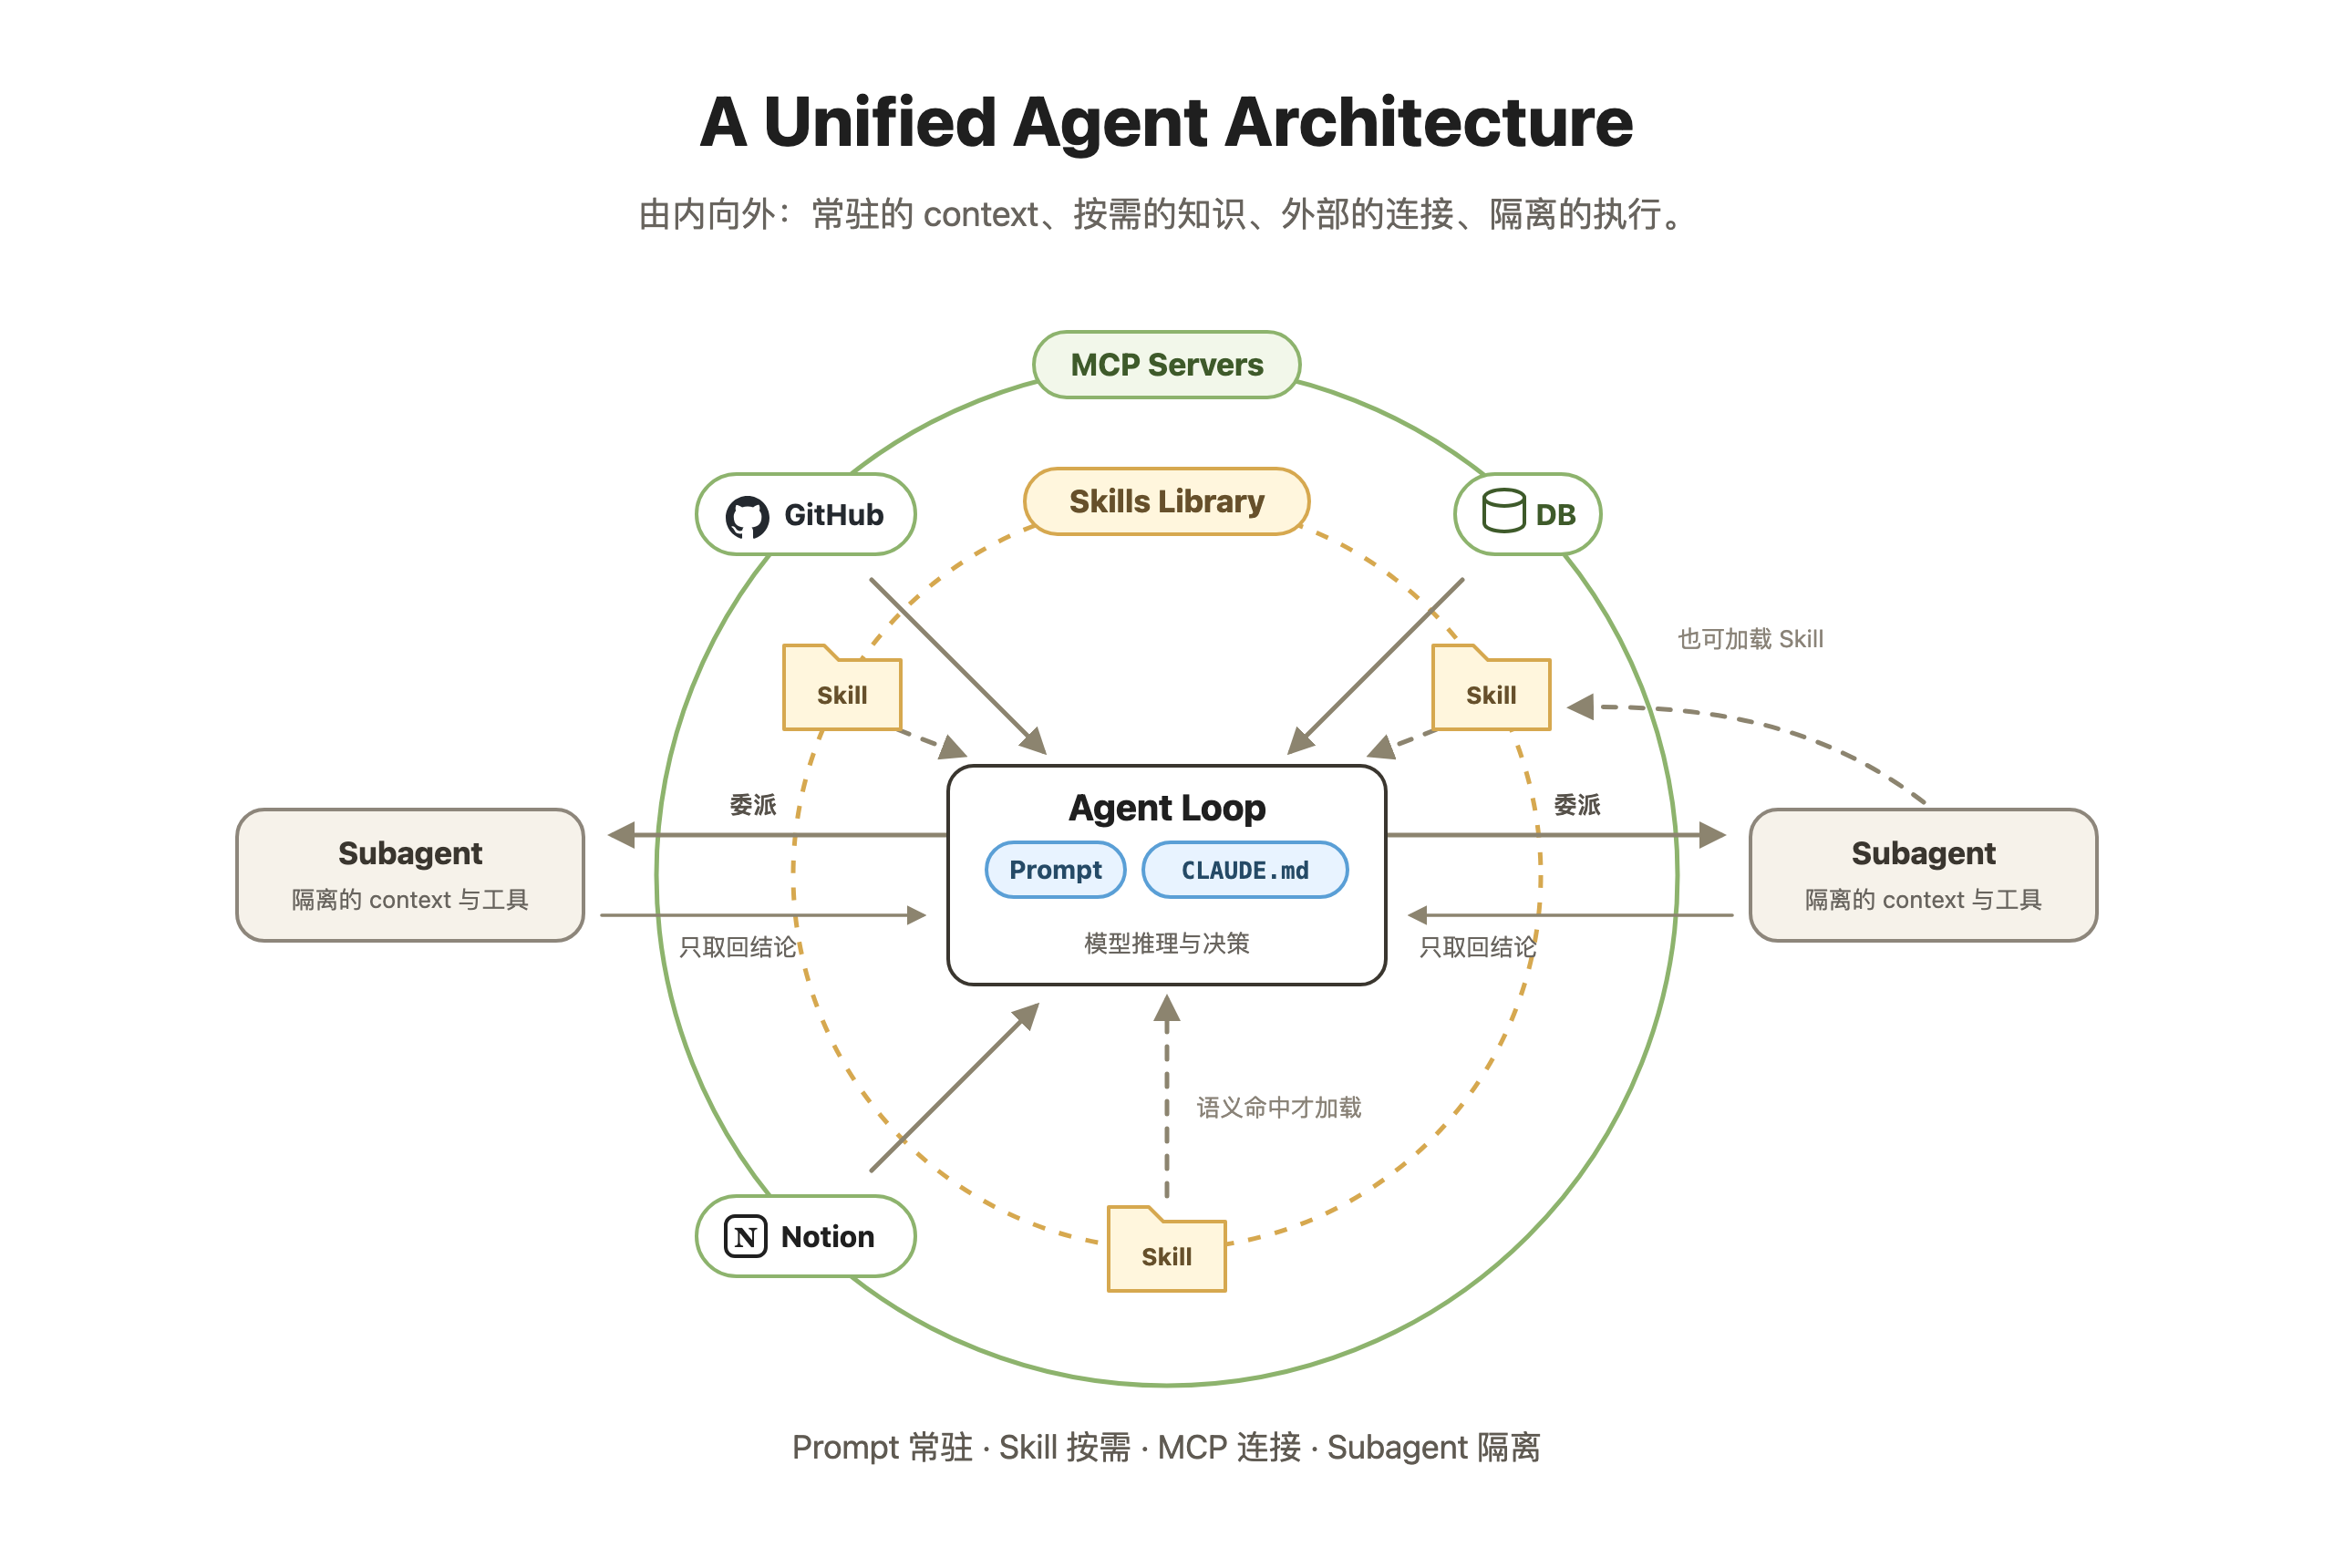
\includegraphics[width=0.82\linewidth]{assets/skill-agent-architecture-overview_gemini_v2.png}
\end{center}

那如此多的概念如何联系在一起？其实其中大部分概念都由 Anthropic 提出，我理解他们的 vision 是\textbf{未来所有的解决方案都应该是 General Agent OS (Claude Code like) + Agent Skills + MCP}。

他们认为给 Agent 加一个新领域的能力，往往就是两件事：配好该用的 MCP，装好该用的 Skills。他们自己也确实在按这个叙事推出行业方案：生命科学方向的 \weblink{https://github.com/anthropics/life-sciences}{life-sciences}（repo 建于 Skills 发布次日，配合 Claude for Life Sciences 上线）和金融方向的 \weblink{https://github.com/anthropics/financial-services}{financial-services}，每个\textbf{“产品”}就是打包好的一组 MCP 加一组 Skills，外加少量 Agent 定义。

简单总结：Prompt 和 \code{CLAUDE.md} 是人主动塞给模型的 Context；MCP 负责连接外部世界；Subagent 负责把复杂任务拆出去、隔离上下文。Skill 的特别之处是把两件事一起做了：\textbf{既装着程序性知识，又自带按需加载的取用方式}。

% ---------------------------------------------------------------- Section 3
\section{Why do we need Skills?}

前两节回答了 Skills “是什么”。这一节会更强调“为什么”：\textbf{为什么是现在，为什么是这种形态？}

Skills 团队自己讲过一个很形象的类比：报税这件事，你会交给 300 IQ 的数学天才，还是一个经验丰富的税务专家？Barry 说他每次都选后者，没人想让天才从第一性原理现场推导 2025 年的税法。\textbf{今天的 Agent 很像那个天才：聪明，但缺少你所在领域的专业经验。}

目前模型的基础智能越过了阈值，Agent 缺的是\textbf{程序性知识}。程序性知识塞进一段长 Prompt 或 Context 文件，也能起到类似的效果（内容本身从来不是 Skills 的创新）；Skills 解决的是它的工程问题：放在哪里、什么时候被加载、怎么跨会话复用、怎么分发给整个团队。就像人不会背下整个图书馆，靠的是索引和目录。这才是 Skills 和一段普通 Context 之间真正的区别。所以 \textbf{Skills 是 Anthropic 给出的、注入这种知识的标准做法}。Skills 自发布后，很快被 OpenAI 等同行采纳为标准，这也有助于 Skills 和 Agent 共同进化，完整论证放在 Appendix A。

\subsection{通用 Agent 的崛起}

过去大家很自然地认为：不同领域需要不同 Agent。法律 Agent、财务 Agent、科研 Agent，各有自己的工具、System Prompt 和工作流。这个思路看起来合理，因为每个领域的任务差异确实很大。

\begin{center}
  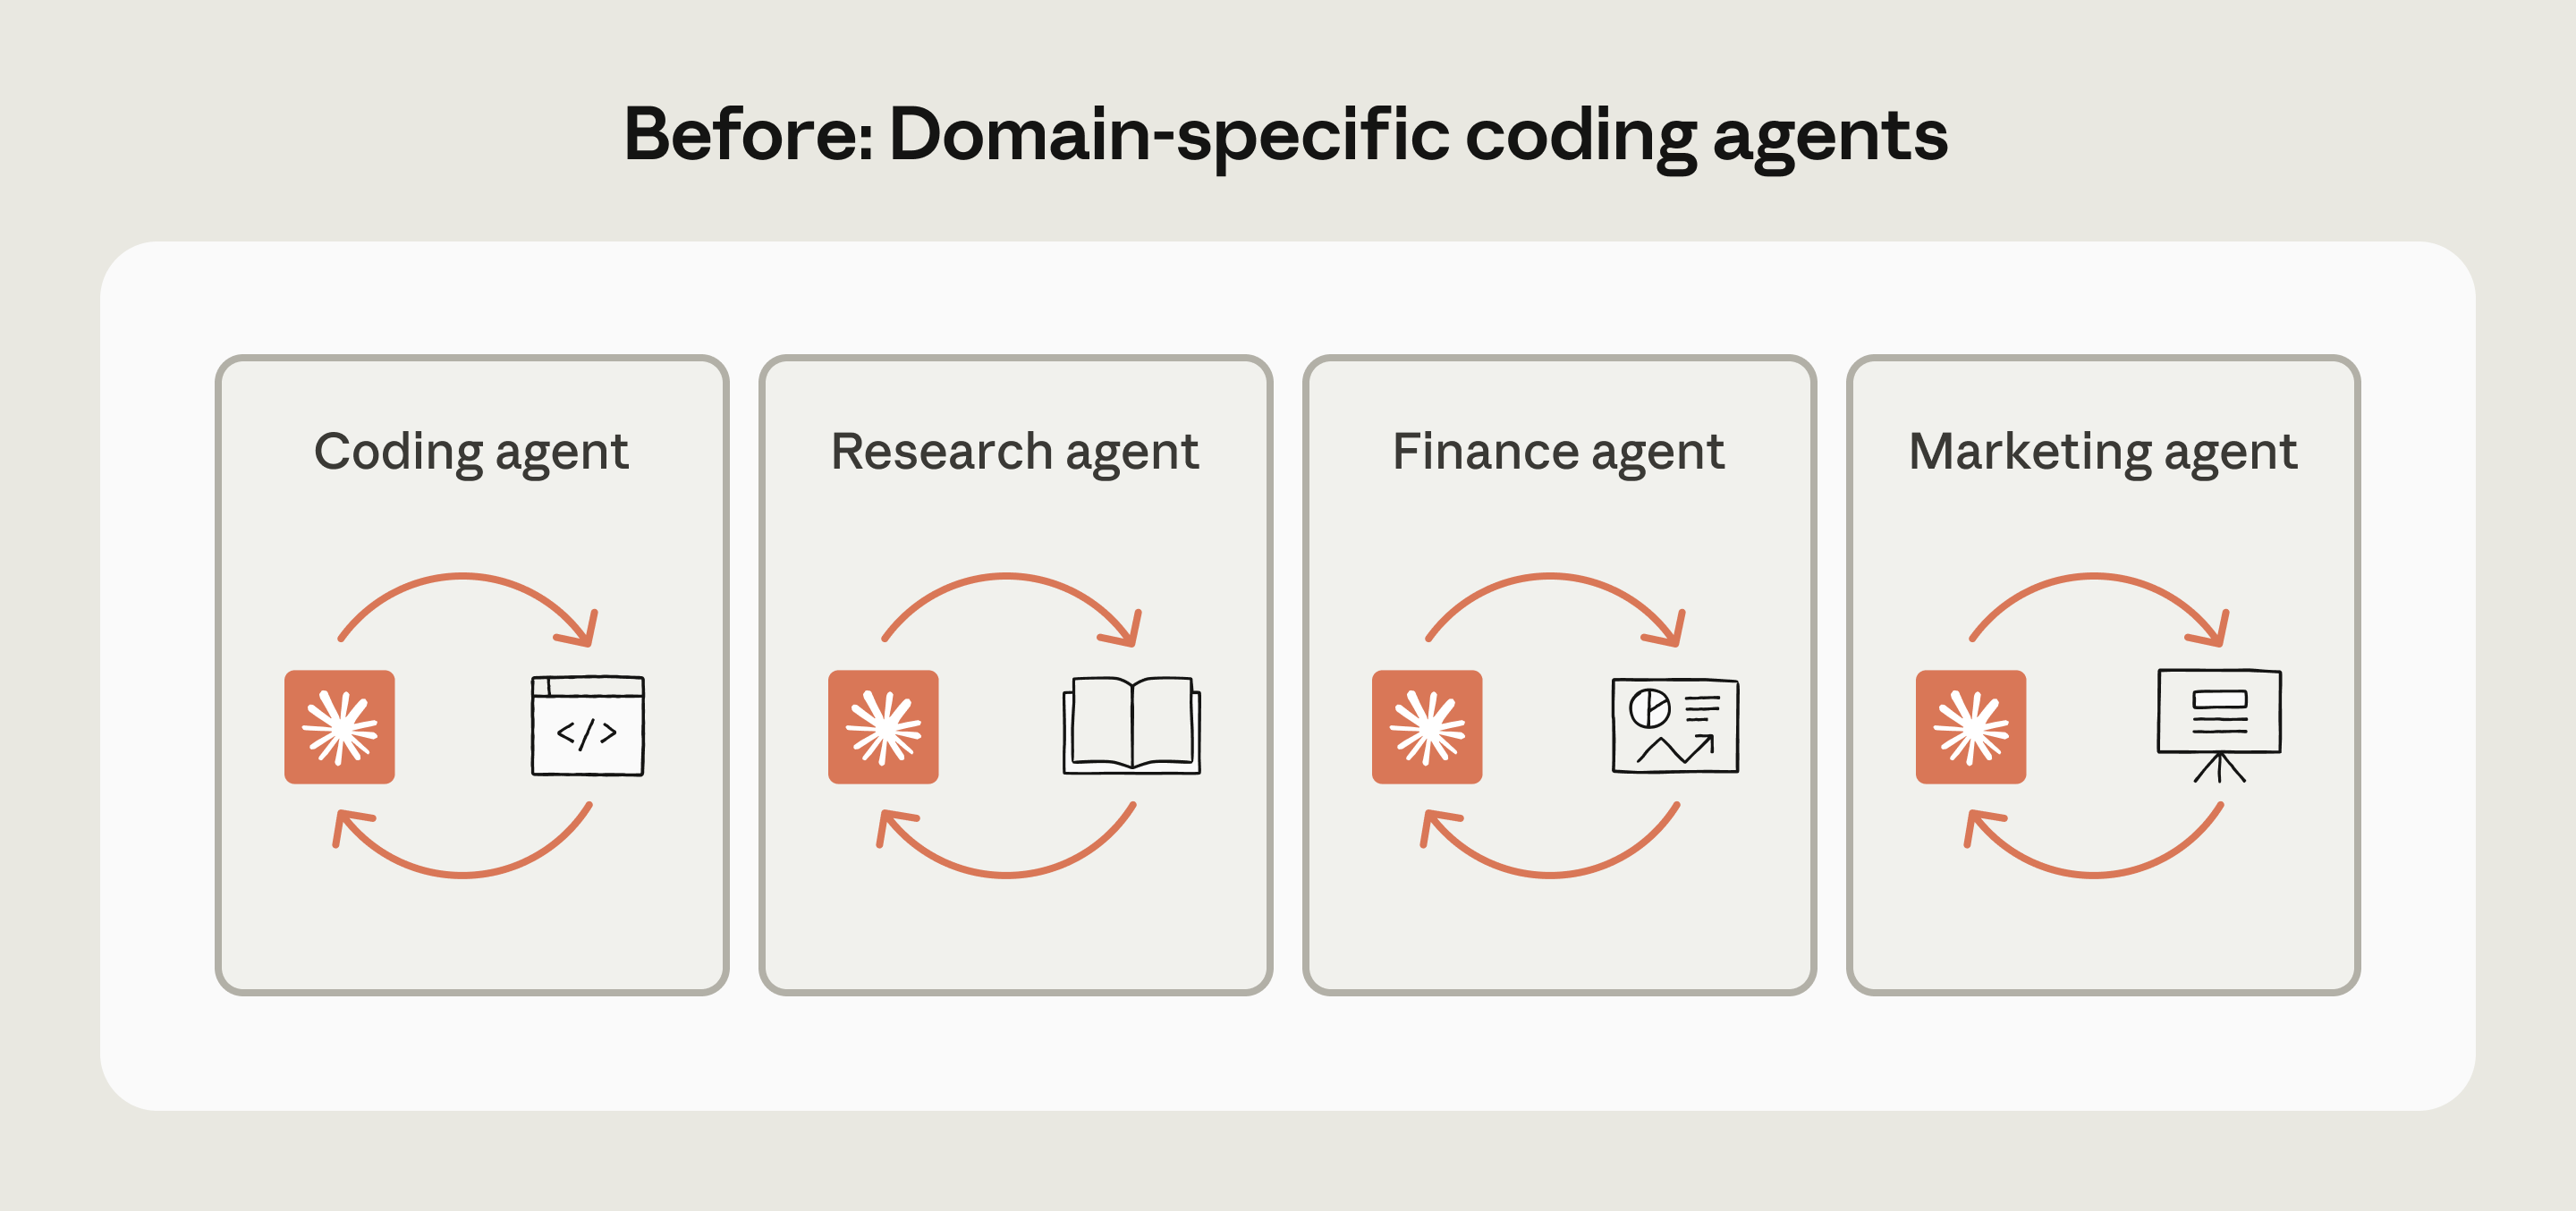
\includegraphics[width=0.8\linewidth]{assets/building-agents-fig1-before.png}
\end{center}

但 Anthropic 基于 Claude Code 的经验给出了另一个判断，并且 Codex 随后发扬光大：

\begin{importantbox}[Code is all we need]
我们过去以为不同领域的 Agent 会长得很不一样，每个都需要自己的工具和脚手架。但\textbf{底层的 Agent 其实比我们想象的更通用}。我们发现，\textbf{代码不只是一个用例，而是通往数字世界的通用接口}。\textit{“We used to think agents in different domains will look very different. Each one will need its own tools and scaffolding... Well, customization is still important for each domain. The agent underneath is actually more universal than we thought. What we realized is that code is not just a use case but the universal interface to the digital world.”}
\end{importantbox}

一个财务报告任务，表面看和写代码无关。但 Agent 可以通过 Tool call（API 或 MCP）拉数据、用 Python 做分析、用代码生成图表，最后生成报告。如果再加载几个财务相关的 Skills（\weblink{https://github.com/anthropics/financial-services}{financial-services}）和视觉设计相关的 Skills（\weblink{https://github.com/anthropics/skills/blob/main/skills/frontend-design/SKILL.md}{skills/frontend-design}），你可以在 30 分钟内拿到一份专业级的 report。

此时限制你的不再是个人时间：只要有足够的 tokens，你可以轻松并行 10 份报告，tokens 直接换算成 workforce。营销方案也类似：从 CRM 抓客户数据、跑分析脚本、生成 slide 和 brief。尽管领域不同，Agent 用的基本工具是同一套：\textbf{终端、文件系统、代码执行，加上几个外部 Tool / API}。我现在的 codebase 里就有大量 Automation 在帮我做各类任务。

\begin{center}
  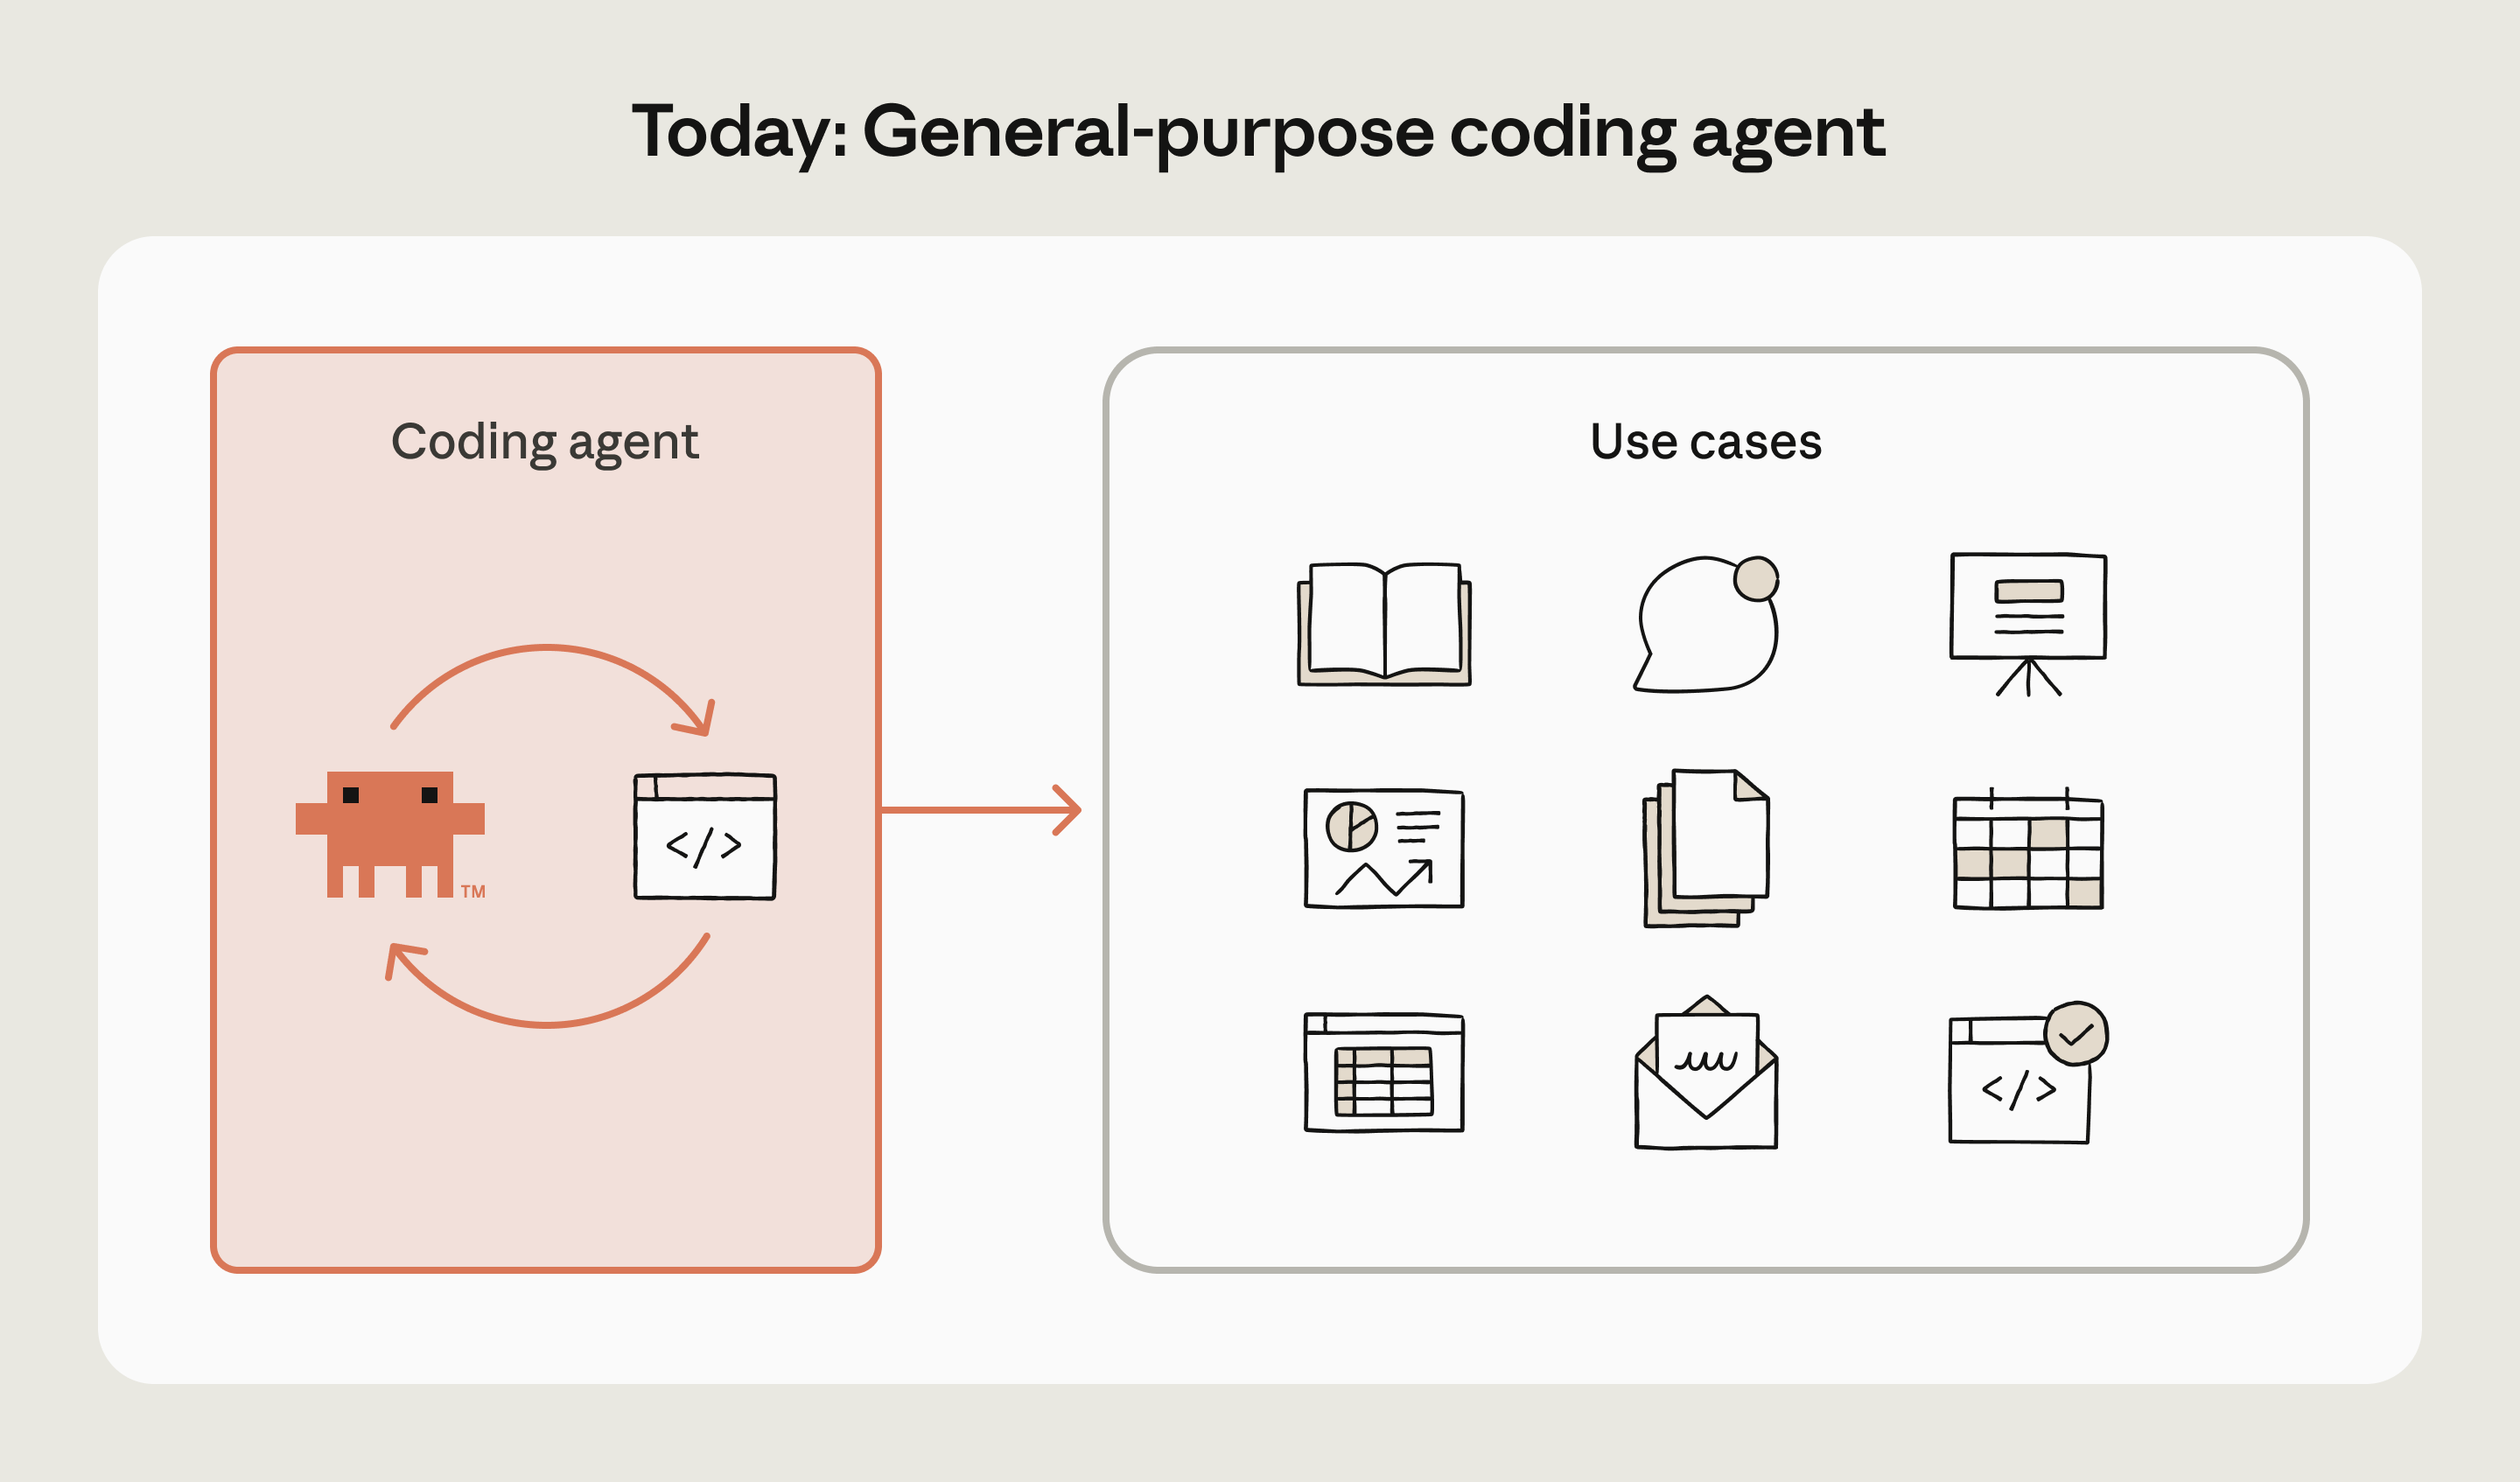
\includegraphics[width=0.8\linewidth]{assets/building-agents-fig2-today.png}
\end{center}

从过去为每个领域精心构建一套 Agent loop，到现在 Coding Agent 涌现出解决各种任务的通用能力，我个人感觉\textbf{关键是在模型基础智能达标后，其 Agentic 能力也迈过门槛}。（反例是 Gemini 3.1 Pro 这个模型，Agent 能力严重拖累模型智能）

Claude Code 首先证明了 Coding Agent 可以承担通用任务（大致从 Opus 4.0 系列开始），我用它写博客、写代码、做调研、购物分析、金融投资。Codex 则更进一步，把 Coding Agent \textbf{显式“改造”成通用工作台}，提供了更多解决 more than code 任务的插件和设计，也比 Claude Desktop 更早长成我心目中通用智能体工作台的样子。我倾向认为 \textbf{General Agent Harness 会越来越热门}，越过 Coding Task 的边界，延伸到任何与认知（Cognition）相关的活动中（推荐观看 \weblink{https://www.youtube.com/results?search_query=aiascent+2026}{AI Ascent 2026}）。

当底层 Agent 足够通用，工程重点自然从\textbf{为每个领域造一个新 Agent}，转向\textbf{给同一个通用 Agent 装上可插拔的专业知识}。这和 Push $\to$ Pull 是同一个趋势：Agent 越通用，越需要一种轻量的方式按需加载领域知识，而不是每次都从零开始教。

\begin{center}
  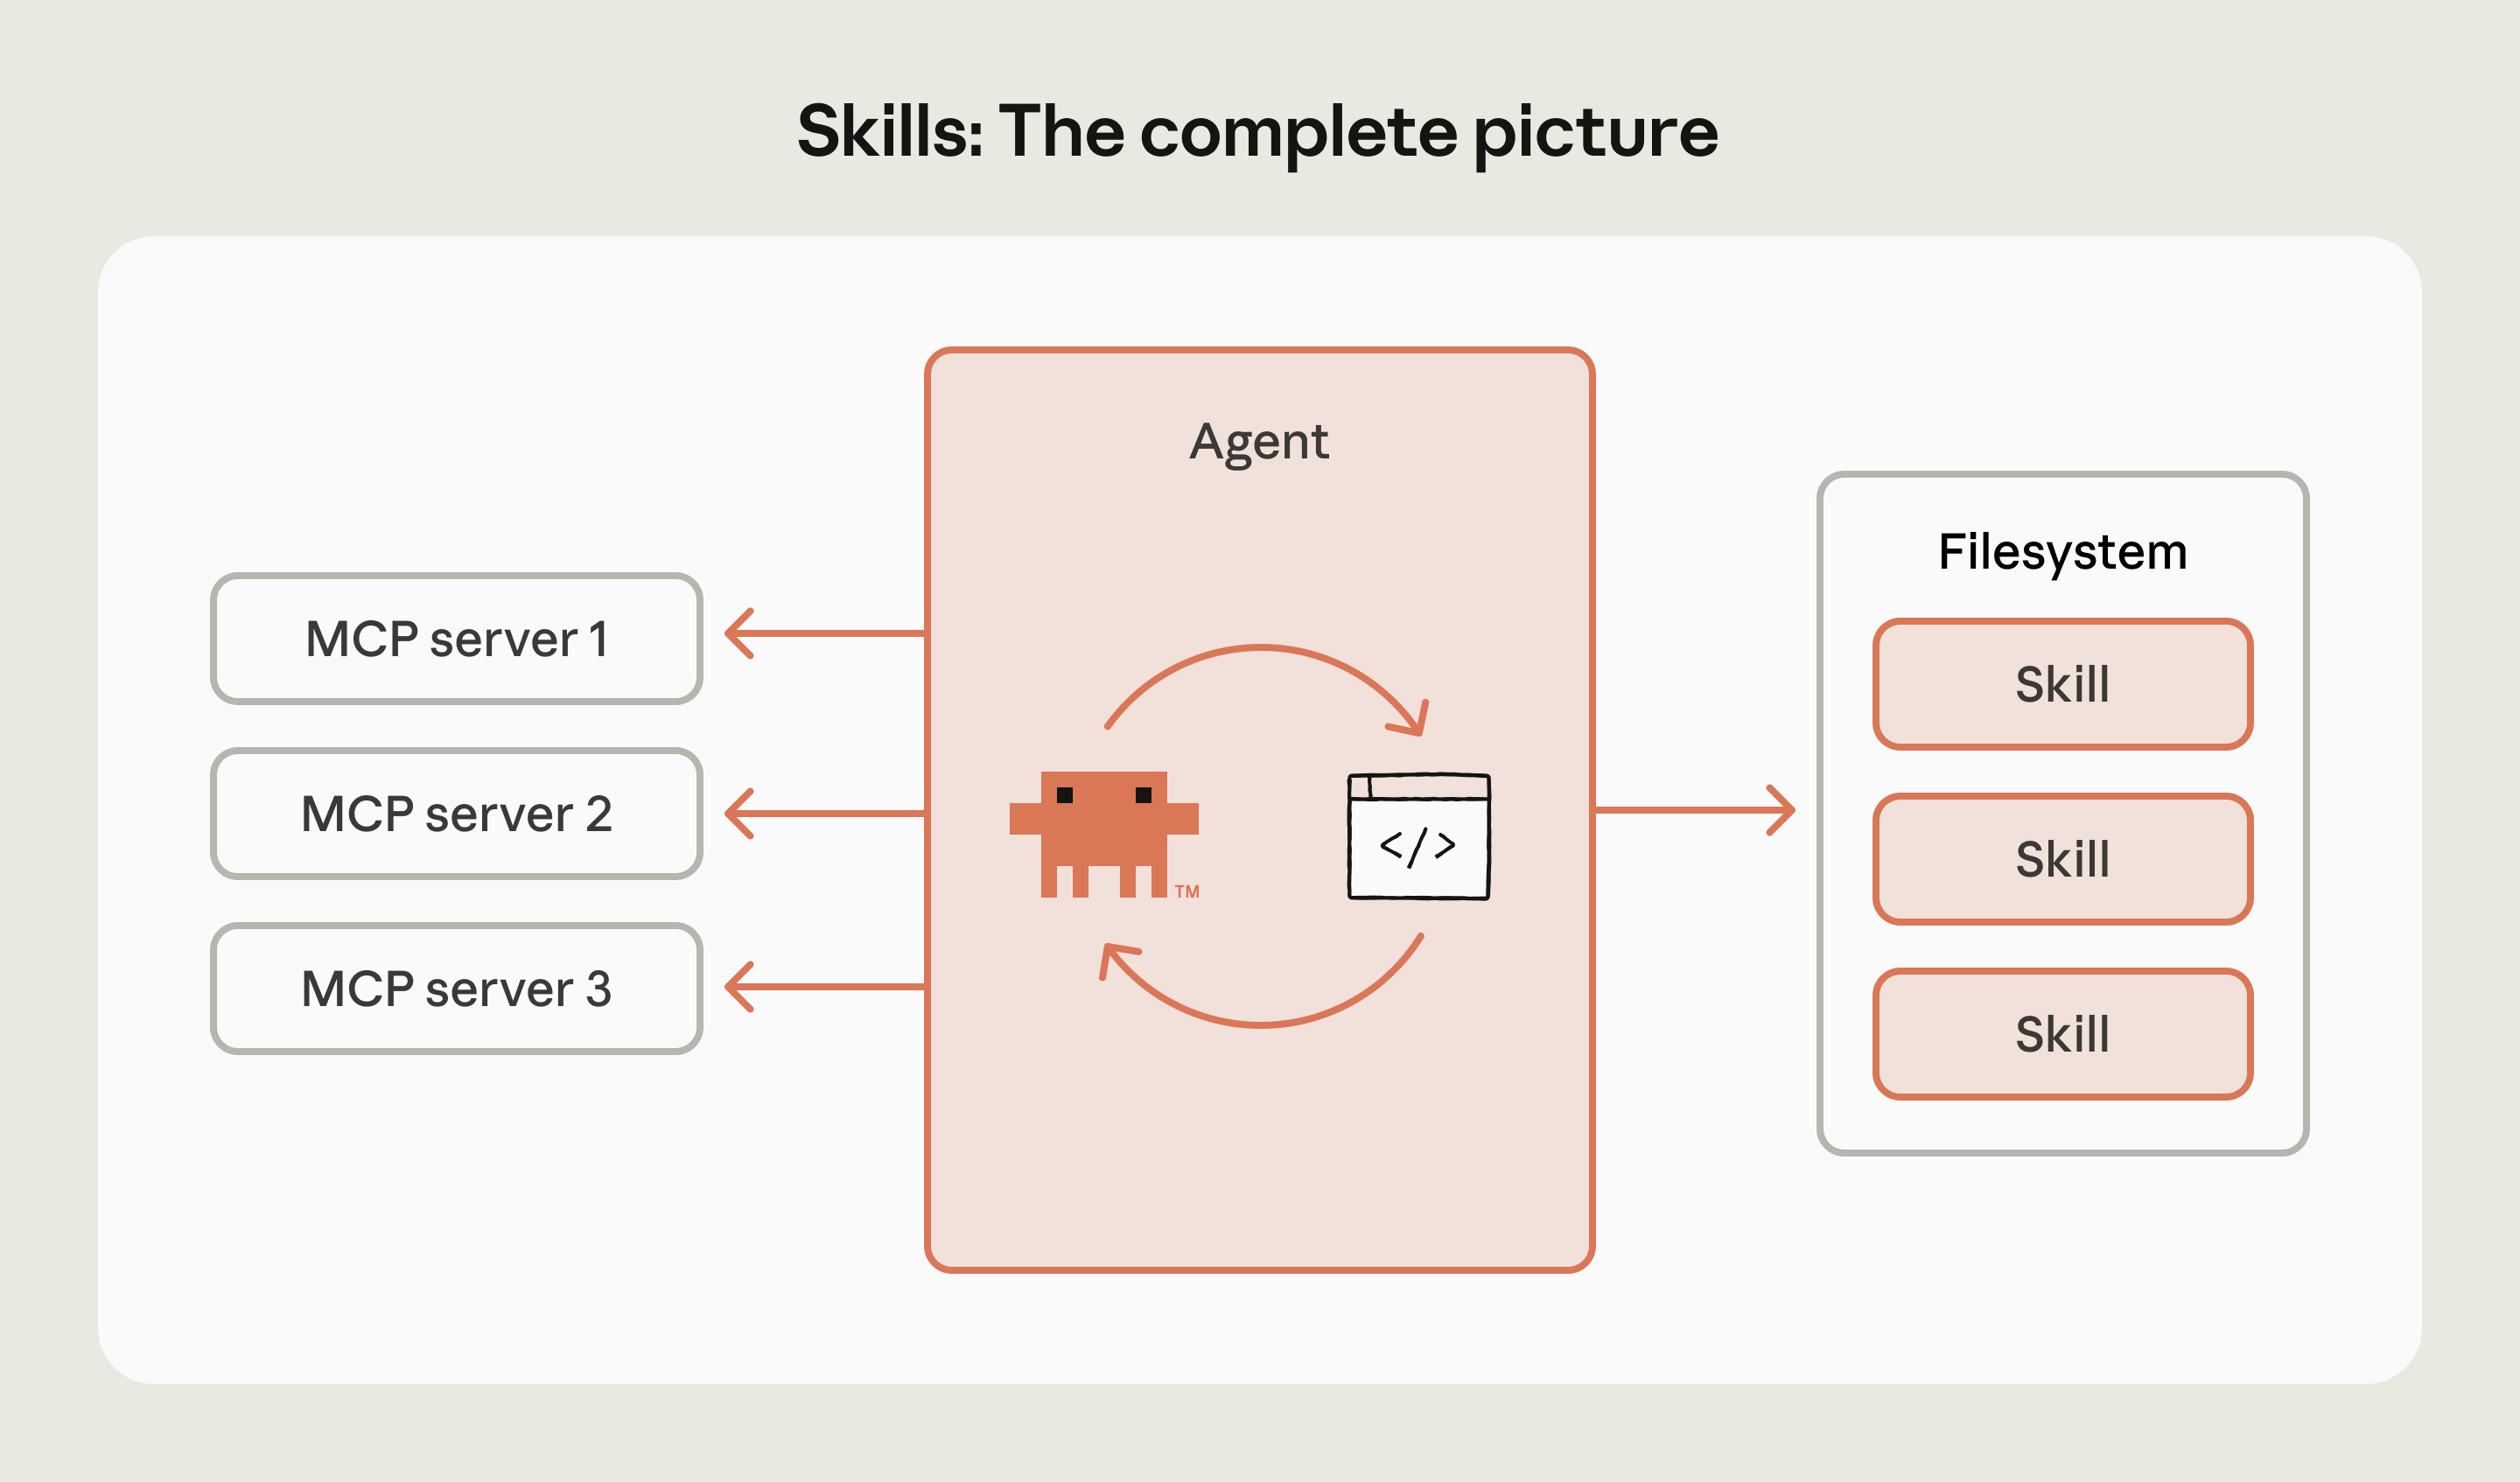
\includegraphics[width=0.9\linewidth]{assets/agent-skills-building-agents-fig3-architecture.png}
\end{center}

\opfig[0.9]{assets/agent-skills-analogy.png}{模型像处理器，Agent Runtime 像操作系统，Skills 是应用层。Source: \weblink{https://claude.com/blog/building-agents-with-skills-equipping-agents-for-specialized-work}{Building agents with Skills}}

\subsection{让 Agent 第 30 天比第 1 天强}

Anthropic 认为 Skills 是\textbf{走向 continuous learning 的一个 concrete step}。这里的 learning 并不是模型参数的更新，指的是让 Claude 写下来的流程、脚本、偏好和失败经验，可以被未来的自己复用。

\begin{blockquote}
Claude 写下来的任何东西，都能被未来版本的自己高效使用。这让学习真正变得可迁移。\textit{“Anything that Claude writes down can be used efficiently by a future version of itself. This makes the learning actually transferable.”}
\end{blockquote}

任务执行中积累的失败模式、用户偏好、验证流程，沉淀为结构化的上下文：标准流程写入 \code{SKILL.md}，可复用代码写入 \code{scripts/}，详细文档写入 \code{references/}。下次遇到同类任务，Agent 无需从头探索，直接从已有经验出发。

\begin{center}
  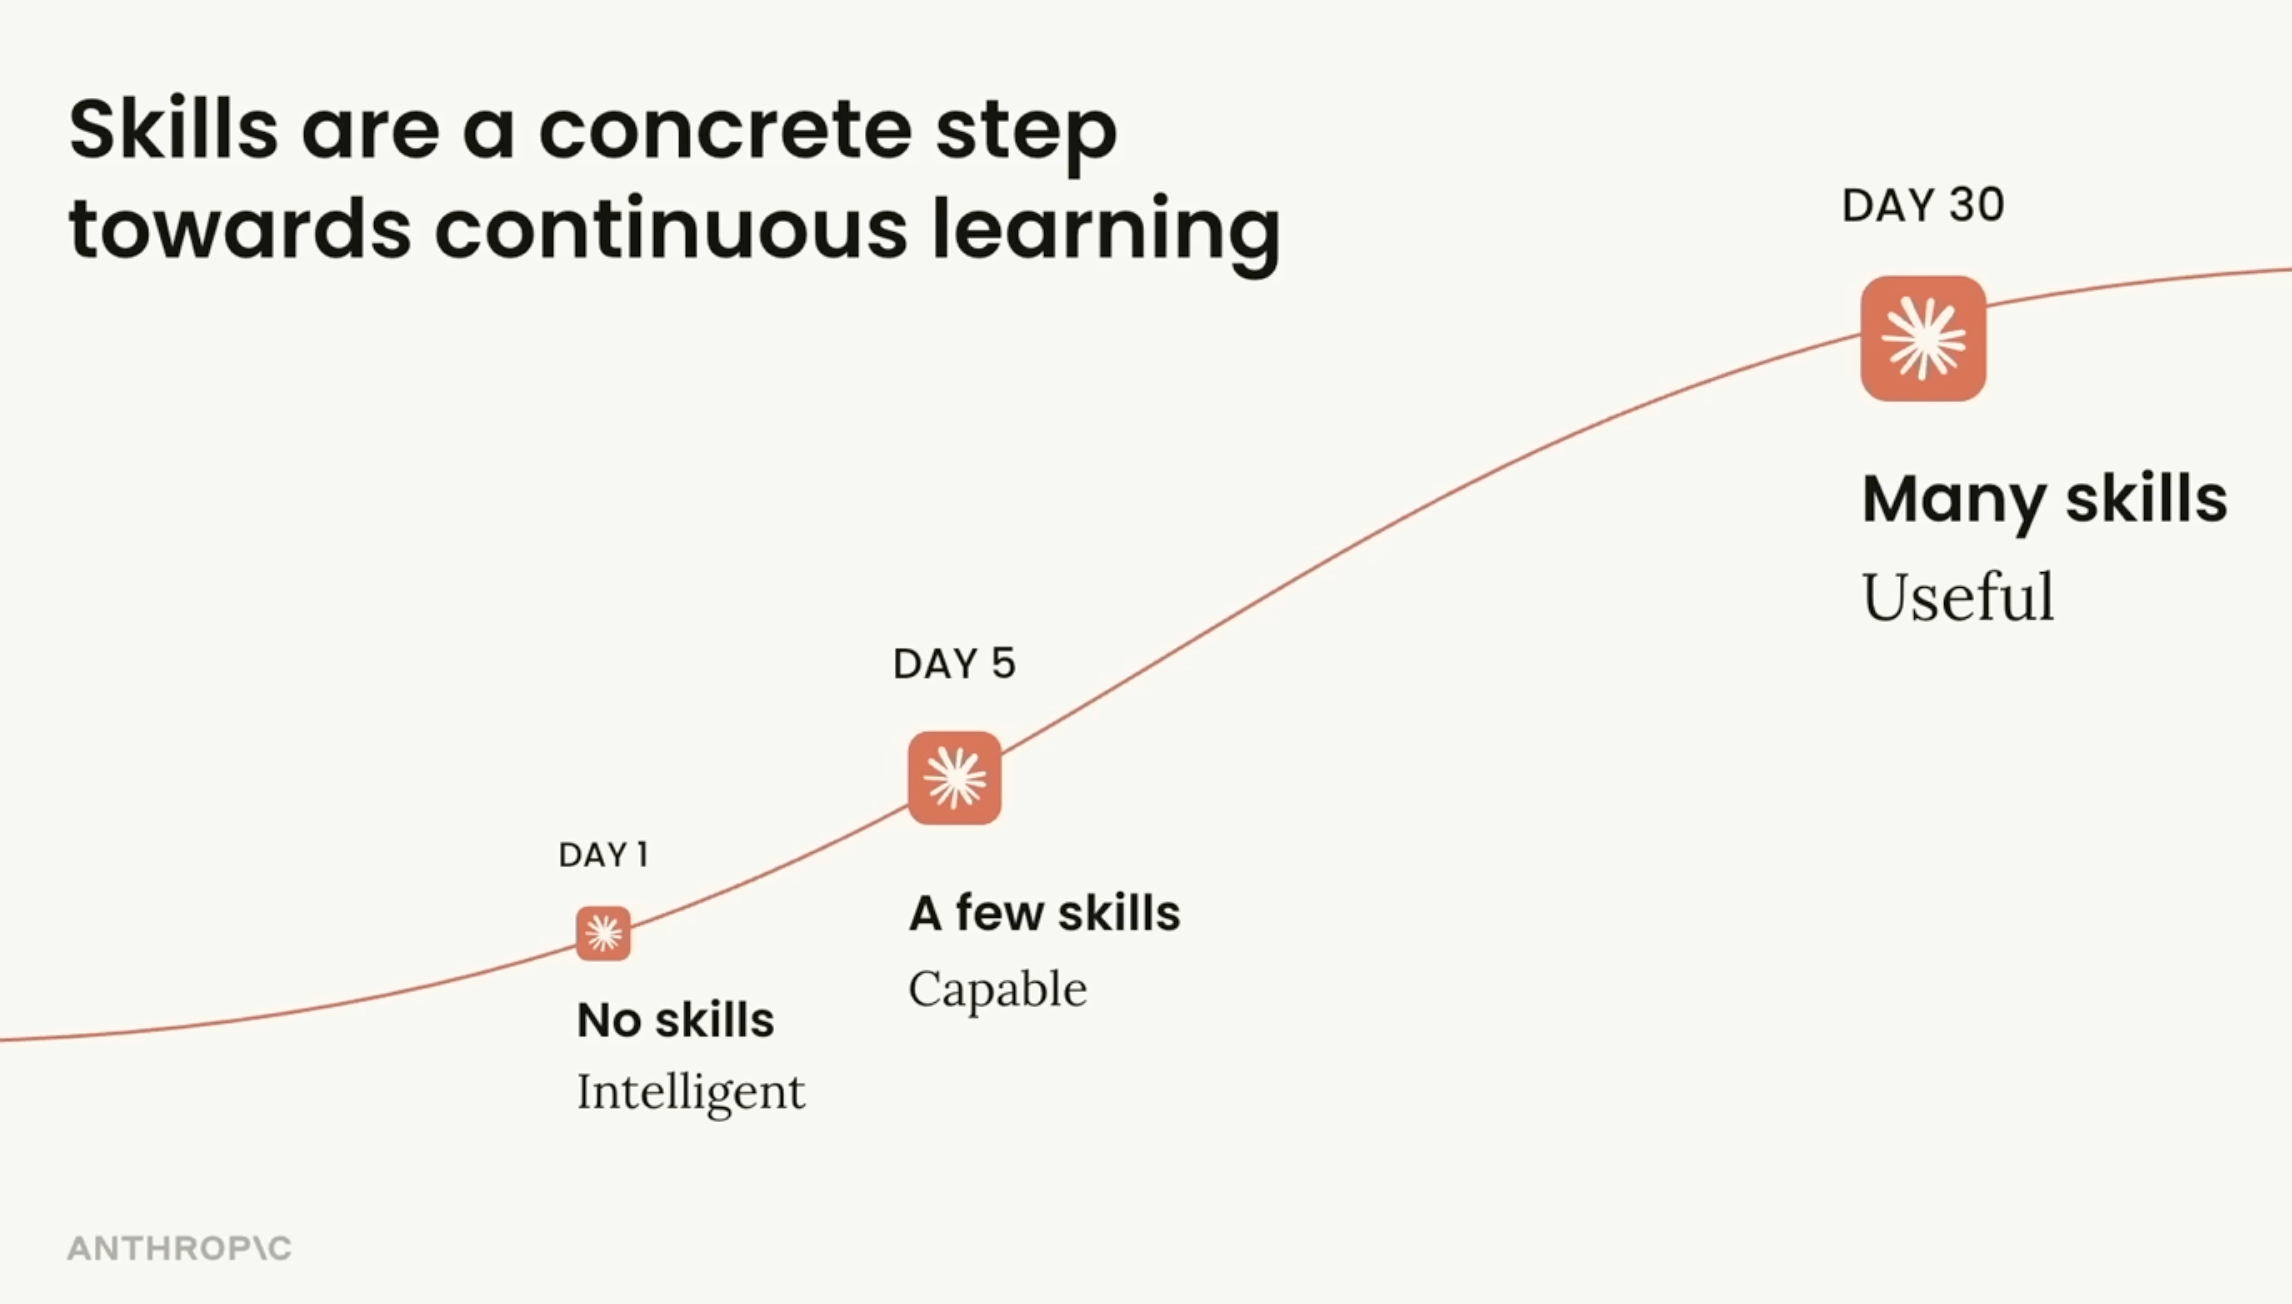
\includegraphics[width=0.72\linewidth]{assets/externalized-continual-learning.png}
\end{center}

我的实践之一是在项目中维护 \code{contexts/} 文件夹，将任务拆分为两个阶段：\textbf{Context（探索）}与 \textbf{Execution（执行）}。Context 任务负责探索问题空间并输出 Context 文件（包括必要的实验性工具调用）；通过在探索阶段投入更多 tokens（explore token scaling），为执行阶段构建更精准的 Handoff 上下文，以期找到更优的实现路径。因为执行阶段涉及大量代码变更，试错成本远高于探索阶段。

执行任务完成后，我会在当前 Session 中要求 Agent 对比实际的执行轨迹与 Context 任务制定的计划：哪些地方出现了偏差，哪些经验值得沉淀，从而更新到 \code{contexts/} 和 Skills 中。因为\textbf{它同时产出了 prediction（Context 任务给出的计划）与 ground truth（真实执行轨迹加上用户反馈），构成了一个可学习的样本对}。这与翁家翌（OpenAI）提出的\weblink{https://trinkle23897.github.io/learning-beyond-gradients/}{启发式学习（Heuristic Learning）}有相似之处，区别在于被更新的不是模型参数，而是 Skills 文件或自动化脚本。

基于解决任务的 Session 进行学习，与让 Agent 凭空直接写 Skills 有本质区别：后者没有 ground truth。

\begin{center}
  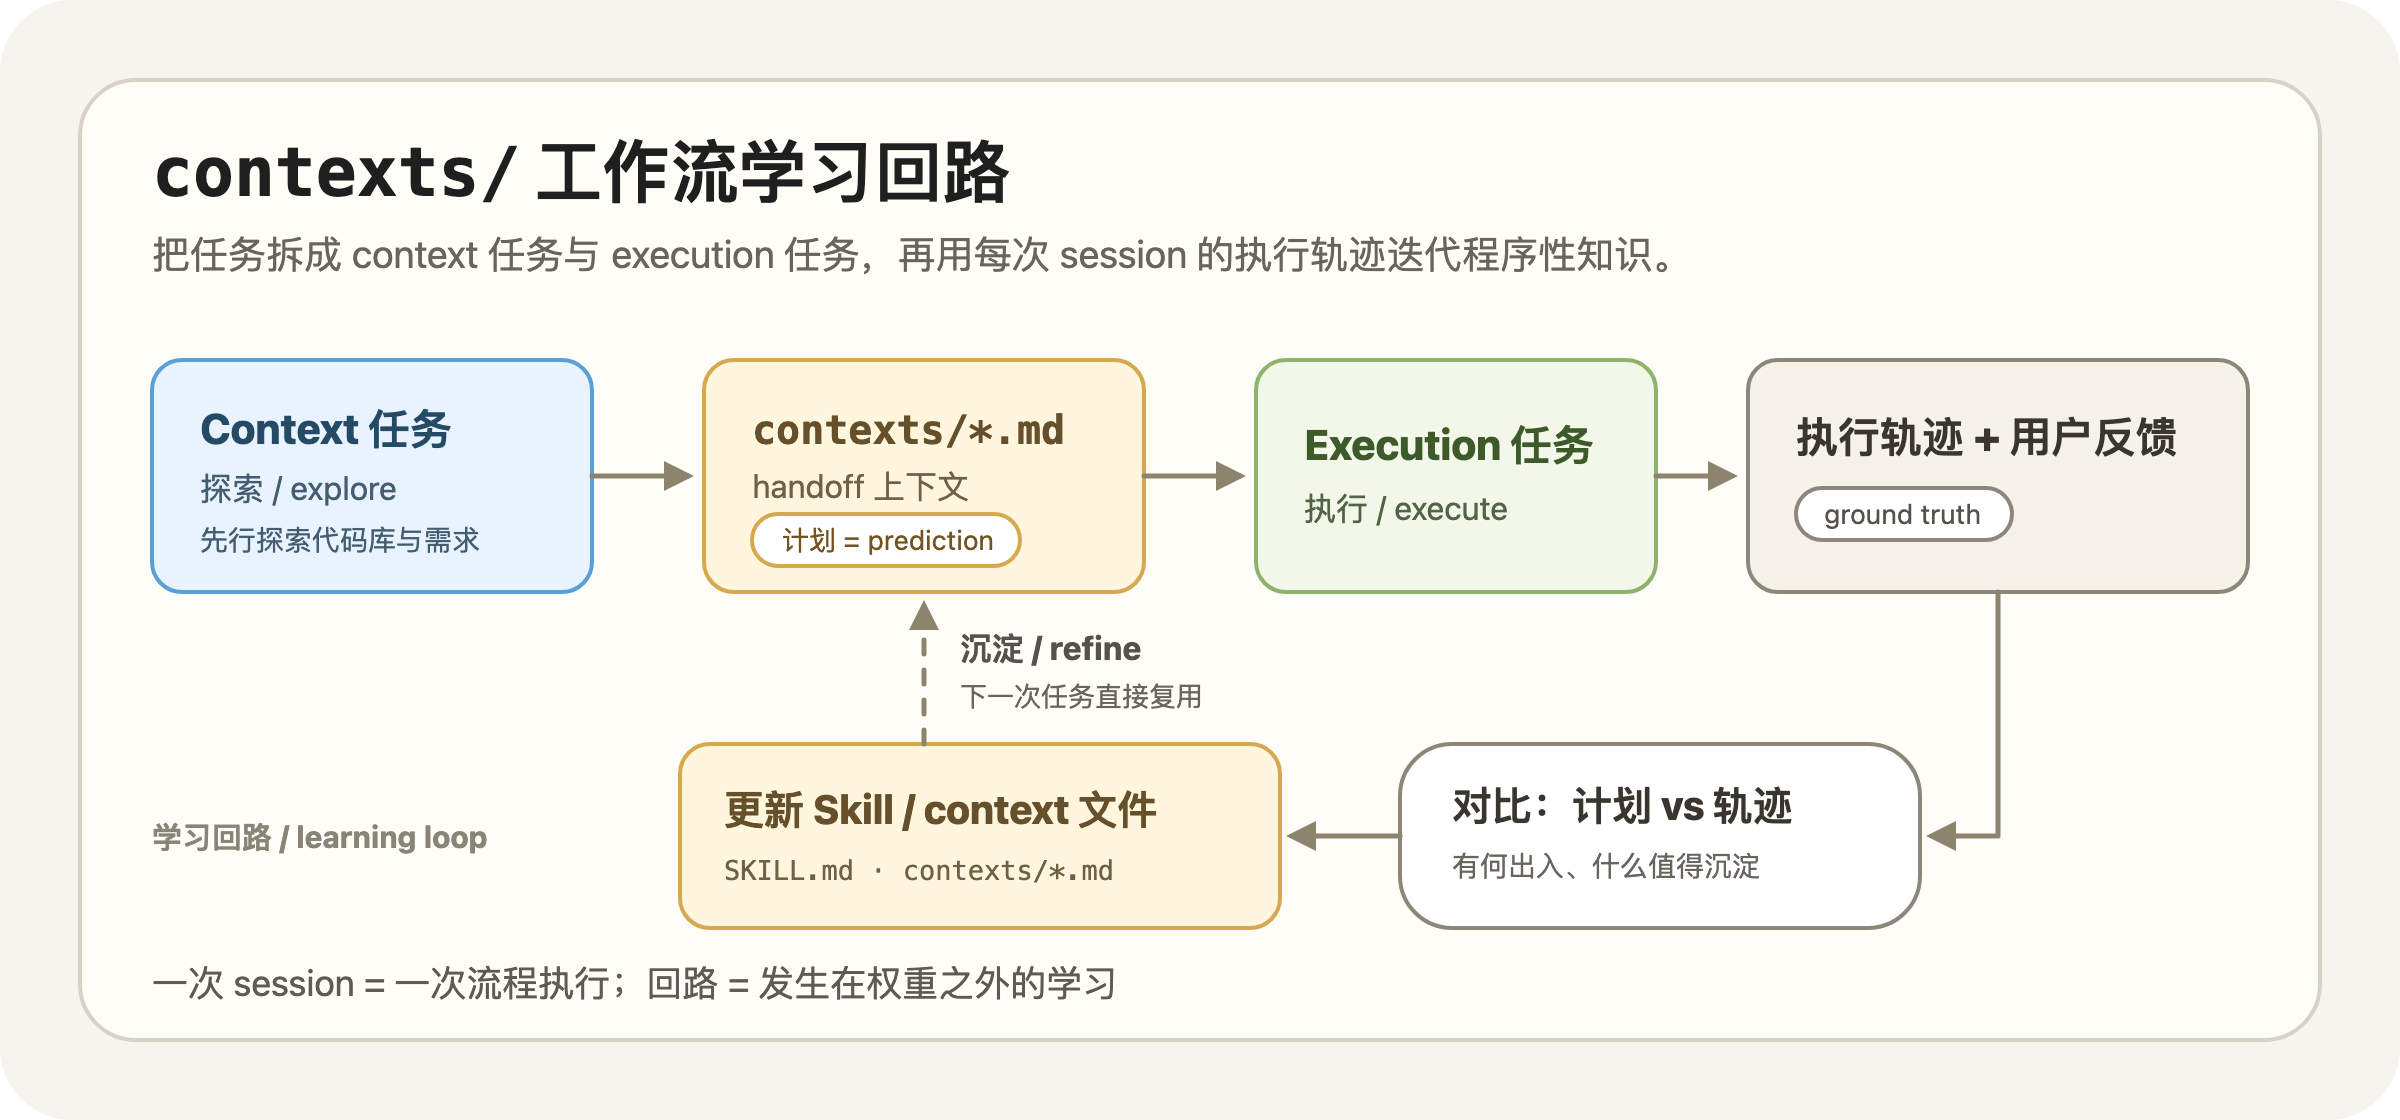
\includegraphics[width=0.9\linewidth]{assets/contexts-workflow-loop_claude.png}
\end{center}

\textbf{为什么 Skills 的更新可以视为持续学习？}

我们把持久化一些结论到 Context 文件的过程视为持续学习，你或许会联想到 2.4 节讨论的 Memory。它是否也构成持续学习？我认为同样可以，两者运行的是相同的回路：Session 中产生信息，后台提取，写入文件，下次注入上下文。从这个角度看，auto-memory 是全自动的持续学习，\code{contexts/} / Skills 工作流则是 human-in-the-loop 的持续学习。差异仍然是 2.4 节归纳的三点，其中我最关注的是\textbf{谁来决定写入的内容}。

对照 RLHF（Reinforcement Learning from Human Feedback，基于人类反馈的强化学习）的框架进行思考。RLHF 的核心流程是：模型产出行为，人给出反馈，反馈转化为奖励信号，更新模型，改善下一次行为。Skills 学习的工作流运行的是相似的流程：一次 Session 对应一次行为，\textbf{计划与实际的偏差，加上我的评价}构成了人类反馈。区别在于更新的机制：RLHF 将反馈蒸馏为 reward model，再去更新权重；而在这套工作流中，反馈由人直接筛选，被更新的是那份描述流程的文件（Skills）。学习的载体从模型权重变成了 Context 文件。这也为 Appendix D 中 SkillsBench 的实验结果（\textbf{模型自写自用，提升接近于零}）提供了一种解释：RLHF 的反馈来源是人，让模型自行编写 Skill 并自行使用，相当于将人从回路中移除。

从形态上看，学习的产物本质上是压缩。一次 Session 的轨迹可达数万至数十万 tokens，合并回 Skill 往往只是几行改动；数十条任务执行的轨迹沉淀下来，可能仅凝结为一份几百行的 \code{SKILL.md}。Context Engineering 篇中引用过 Ilya Sutskever 关于“压缩即智能”的观点，我认为这里是同一个逻辑：将长轨迹压缩为短的启发式结论。

因此 Anthropic 对 Skills for learning 的愿景是：Day 1 的 Claude 只具备通用知识；Day 30 的 Claude 如果能读取沉淀下来的 Skills，则可以了解团队偏好的格式、常用工具链、内部流程，以及容易出问题的环节。它不需要记住一切，关键在于\textbf{在正确的时机取回正确的经验}。因此 Skills 是 Harness Engineering 中不可或缺的一环：通过不断迭代，我构建的 Skills \& Hooks 可以帮助我从零构建起几十万行的项目，并在其中高效并行多个任务，我的思考预算只需要花在少数真正需要深入的问题上（推荐阅读：\weblink{https://openai.com/index/open-source-codex-orchestration-symphony/}{OpenAI - An open-source spec for Codex orchestration: Symphony}）。

\begin{tipbox}
这也是个人开发者在 Harness Engineering 上需要优化的部分。我目前的经验有两条：在 Harness 设计阶段投入越多，后续开发阶段的效率越高；以及要不断扩展自己效率的边界，尽可能让你的 tokens 并行化（Subagent）、自动化（Automation / Loop）。
\end{tipbox}

% ---------------------------------------------------------------- Section 4
\section{How? Best Practices for Building Skills}

怎么写好一个 Skill，Anthropic 自身的教程已经相当完整，推荐阅读 \weblink{https://platform.claude.com/docs/en/agents-and-tools/agent-skills/best-practices}{Best Practices} 和 \weblink{https://claude.com/blog/complete-guide-to-building-skills-for-claude}{Complete Guide} 这两份文档。更 AI-Native 的做法是：将链接直接提供给 Coding Agent，让它据此 Review 你现有的 Skill。

因此本节不复述教程，而是从实践出发，讨论几个我认为值得分享的点。仍沿用本文的两条主线来组织：Skills 本质是 Context，所以先看\textbf{Context 的内容怎么写好}（见 4.1 节）；Delivery 机制是 JIT，再看\textbf{结构和触发怎么设计}（见 4.2 节）；最后是\textbf{如何迭代与验证}（见 4.3 节），以及具体例子的分析（见 4.4 节）。

在进入最佳实践之前，先思考一个前置问题：什么时候值得写 Skill？Anthropic 给出的标准很清晰：\textbf{“这个任务我已经做过 5 次了吗？以后还会再做 10 次吗？”}（\textit{“Have I done this task at least five times? Will I do it at least ten more times?”}）两个问题都回答是，才值得投入时间。

我自己的标准更偏向 \textbf{Learn by doing，按需沉淀}。对于明显重复的流程，我会先将其提炼为 Skill，在后续同类场景中直接复用。初版通常难以一步到位，因此我会结合 Session 的实际表现进行迭代（即 3.2 节中提到的流程），一般经过两到三轮调整后，Agent with Skills 的表现趋于稳定。官方推荐的起步方式 \textbf{Iterate-on-one-task} 也是同一个思路：先在一个有难度的任务上把单次 Prompt 调通，再将验证有效的指令提炼为 Skill。共同的前提是先有一条成功的轨迹，提炼发生在轨迹之后，而不是凭空设计。

\subsection{怎么写一个好的 Context}

既然 Skills 本质是 Context，那\textbf{怎么写好一个 Skill} 的前半个答案，就在于一份\textbf{怎么写一个好的 Context}。我将其归纳为两个层面：

\begin{itemize}
  \item \textbf{内容层面：已知的不写，未知的写清楚，与当前任务无关的不掺入。}
  \item \textbf{管理层面：保持单一事实来源（Single Source of Truth），维护 Context 文件之间的一致性。}
\end{itemize}

这两条经验均来自与 Agent 协作过程中的教训。内容层面的问题尤为常见：Agent 在生成和更新 Context 时倾向于填充冗余信息，偶尔还会将 Session 中的任务特定内容混入通用文件。而且，它倾向于将 Context 写成\textbf{错题本}式的特例集合，而非可迁移的启发式结论，本质上是一种 hardcoding，相当脆弱。管理层面的问题同样常见：与写代码时类似，Agent 不擅长抽象和归并：同一个结论容易散落在多个文件中，后续更新遗漏一两处，下游 Agent 读到相互矛盾的版本，推理质量随之下降。

关于内容层面，Anthropic 给出的核心建议用一句话概括：\textbf{默认假设模型已经很聪明（“Claude is already very smart”）}。Agent 缺的是在你的项目中，怎么做才算正确。由此推导出一条实用的检验标准：每写完一段 Context，都值得回头问一句：\textbf{这段内容对得起它占用的 token 吗？}冗余的 tokens 会浪费宝贵的注意力预算。

关于内容层面的另一个重要维度是\textbf{指令的精确度}。借用 Anthropic 提到的一个例子：不同任务的解决路径或者说 Agent Action Space 是不同的。可以将任务想象为两种地形：\textbf{窄桥和开阔地}。窄桥两侧是悬崖，容错空间极小，这类任务（如数据库迁移、发布流程）应当将步骤写死，甚至直接提供可执行脚本；开阔地上条条路通终点，只需给出方向和约束，具体路线交由模型判断（如 Code Review 这类高度依赖具体情境的任务）。换言之，\textbf{你给模型留多大的自由度，应当取决于任务本身的容错空间，而非你对模型的信任程度}。分析我自己的 Skills，确实自然分化成了这两类：\code{file-issues}、\code{submit-pr} 等偏向精确步骤，而 \code{db}、\code{web}、\code{core} 开发和自我分析的 \code{principle} 这几个 Skill 则偏向启发式约束。

业界的最佳实践中还有两条建议偏向我所说的 Context 管理。\textbf{一致性}：同一个概念在全文中使用同一个术语，避免让模型去推测两种不同说法是否指向同一件事。\textbf{单一事实来源}：一个结论只在一个位置定义，其他位置通过引用指向它。

\subsection{符合 Just-in-Time Context 的哲学}

结构上的优化，可以对照 1.1 节的三层结构逐层分析。目标是让 Skill 的行为贴合 JIT 的设计哲学：\textbf{触发要精准}，Agent 需要时能可靠加载，不被无关请求误触发；\textbf{披露要渐进}，细节留在 reference files 中按需取用。做不到这两点，Skill 与一段冗长的 System Prompt 没有本质区别。

\textbf{第一层 metadata：控制触发。}\code{description} 是整个 Skill 中影响范围最大的字段：它本质上充当文本分类器，是主 Agent 唯一用来判断是否需要加载的依据。编写它的过程就是在调节漏触发与误触发之间的平衡。Claude Code 团队对此有一个明确的定位：

\begin{blockquote}
description 不是摘要，是“什么时候该触发这个 Skill”的说明。写给模型看。
\textit{“The description field is not a summary --- it's a description of when to trigger this skill. Write it for the model.”}
\end{blockquote}

实操上有四个要点：（1）写清功能和适用场景；（2）包含用户实际会使用的触发短语；（3）统一使用第三人称；（4）出现过度触发时添加负向条件（“Do NOT use for X”）。第三人称是因为 \code{description} 会与其他 Skills 的 metadata 一同注入 System Prompt，“我可以帮你”这类第一人称会造成叙述视角不一致，官方的观察是这会干扰模型对 Skill 的发现和匹配。调试也有便捷的方法：直接询问 Claude \textbf{你什么时候会使用这个 Skill？}，它会复述自己的理解，据此查漏补缺。

\textbf{第二层 body：承载指令。}\code{SKILL.md} 的价值不在于面面俱到，而在于它同时充当\textbf{主流程}与\textbf{路由}：高频路径在正文中写清楚，进阶细节用一句话指向同目录下的独立文件（如“表单填写规范见 \code{forms.md}”），为渐进式披露预留入口。当正文逻辑开始分叉，或能力涵盖多个相对独立的子流程时，首先考虑的不是创建新的 Skill，而是将内容拆分为\textbf{主文件 + 多个 reference files}，我习惯把这些被引用的文件理解成 sub-skill。官方给出的参考线是 \code{SKILL.md} 正文控制在 500 行以内，接近上限时就该拆分。

\textbf{第三层 \code{references/} / \code{scripts/}：支撑按需加载。}reference files 有三条经验。第一，引用只保持一层深度：\code{SKILL.md} $\to$ \code{forms.md} 没有问题，\code{SKILL.md} $\to$ \code{advanced.md} $\to$ \code{details.md} 则有风险，官方的观察是关键信息到第二跳之后容易丢失，模型往往只部分读取。第二，超过百行的 reference 文件，开头附一份目录。第三，多领域的 Skill 按领域拆分文件。\code{scripts/} 则只有一条核心原则：\textbf{代码的执行是确定的，自然语言的理解不是}，能在脚本中完成的逻辑，不应交回给模型去解释执行。

\begin{notebox}[一份复杂的领域知识，应当组织为一个 Skill + 多层嵌套的 \code{references/}，还是拆分为多个独立 Skill？]
前者结构简单、触发统一，但 \code{SKILL.md} 容易随时间/任务膨胀，逐渐退化为全量加载，甚至不得不多层嵌套；后者每个 Skill 小而精准，但会引入两个新问题：如何做最佳拆分、如何避免 \code{description} 定义有重叠。目前有些 Harness 支持 Plugin 的形式，但这个规范并未推广，所以我觉得这一问题还有待演进。
\end{notebox}

\subsection{Eval 是闭环的关键}

为什么 Skill 需要测试？其实我觉得 Agent 时代，测试（Verify / Eval）比生成更重要。对于 Skills，我认为有两个原因：

\begin{enumerate}
  \item \textbf{防退步 / 性能 Regression}：3.2 节把更新 Skill 称作学习，学习就可能学错，改完一版到底变好还是变坏，需要一组固定的测试用例来回答，不能靠体感。通常情况下，大型系统都有多个维度的回归测试（regression test）来捕捉更新带来的潜在性能问题。
  \item \textbf{能力追踪 / capability tracking}：模型每升级一次，都会有一些 Skill 从补充 Agent 能力变成阻碍 Agent，定期跑一遍用例，才知道哪些 Skills 可能不需要了（without skills 也能完成任务）。
\end{enumerate}

实操中值得关注的工作流是 \textbf{Claude A / Claude B 双实例}：A 负责设计 Skill，B 在干净的上下文中测试，避免自我确认偏差。

\begin{center}
  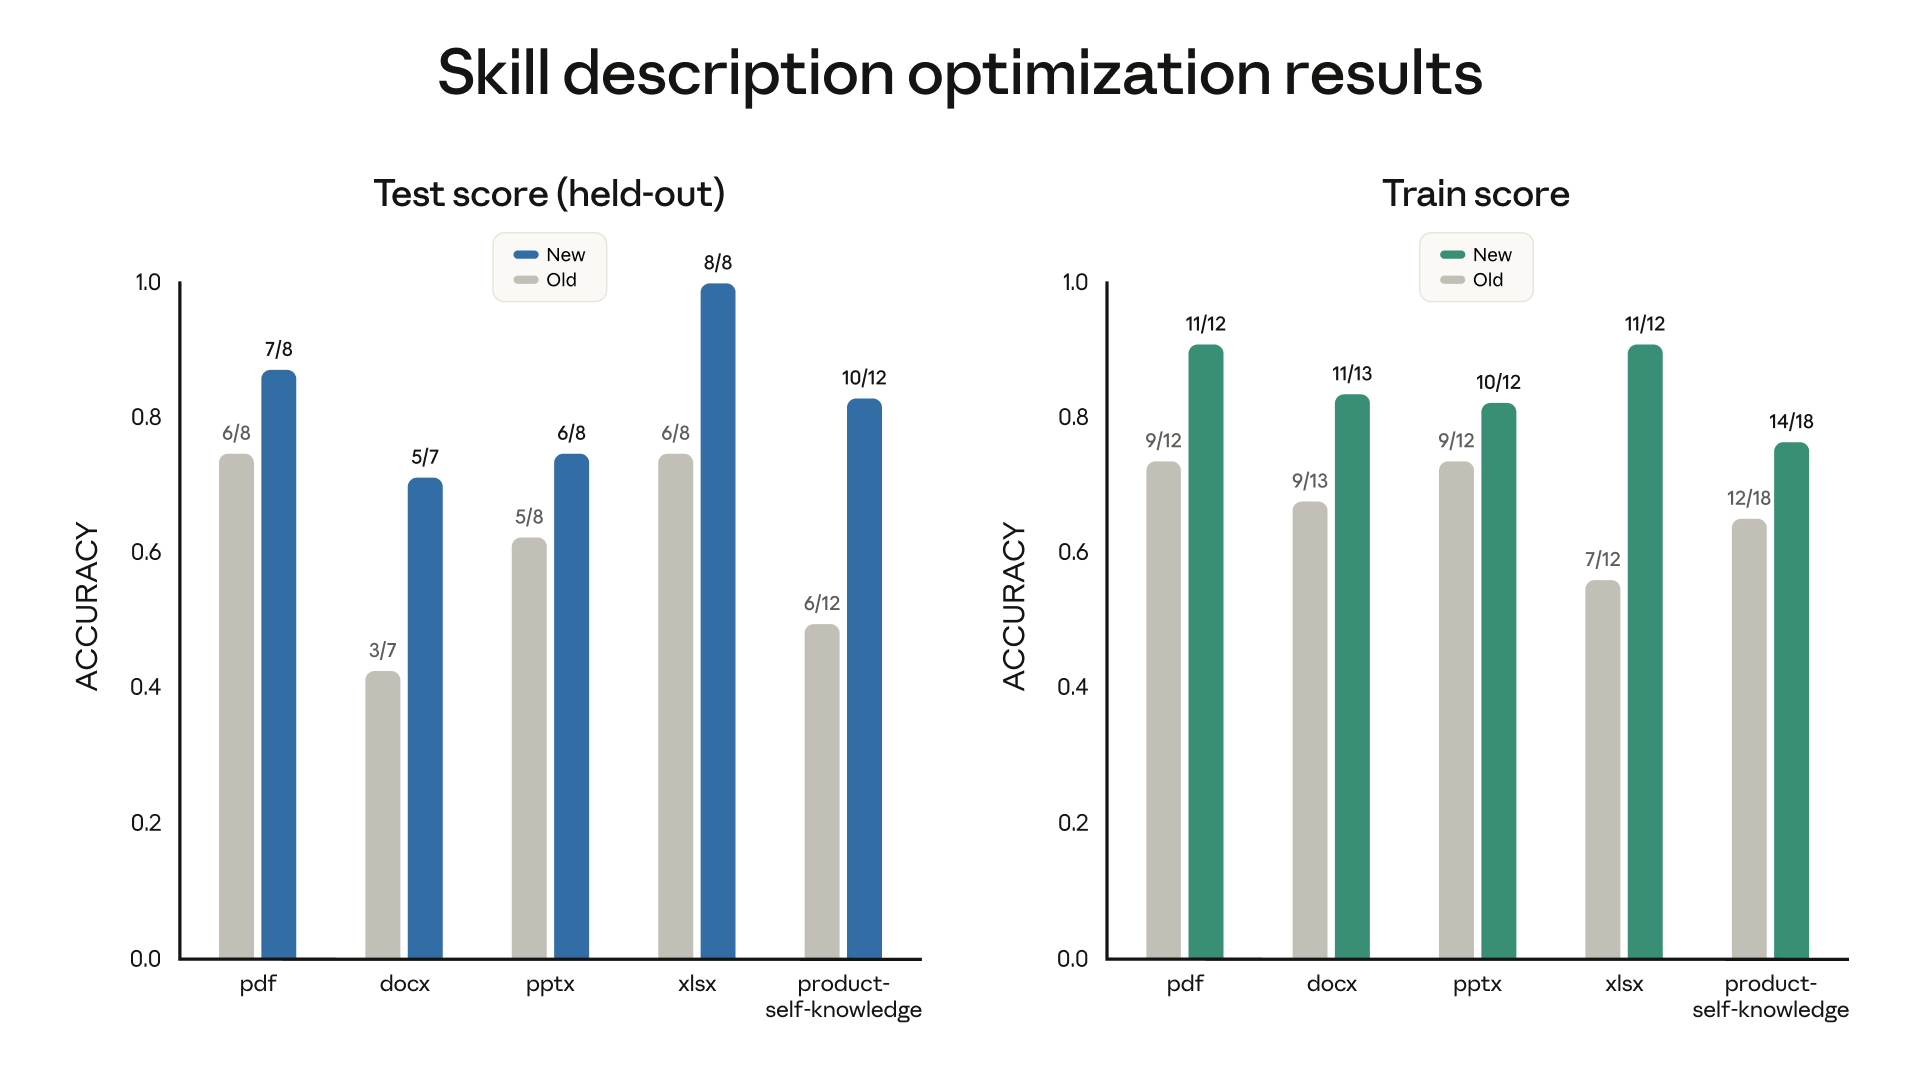
\includegraphics[width=0.92\linewidth]{assets/skill-creator-description-optimization.png}
\end{center}

上图展示了 skill-creator 优化 \code{description} 的实测效果。图中涵盖 5 类文档对应的 Skills，经过 \code{description} 调整后，在 held-out 测试集上均获得了触发准确度的提升。基于这个数据可以推导得到：\textbf{Skills 触发相关的问题是可 Eval、可优化的}。至于更具体的方法论（Eval 如何构建、测试集如何划分、跨模型测试与盲测 A/B 如何执行）属于进阶内容，为了不影响阅读流畅性，我这里也渐进式披露给大家：建议参阅 \weblink{https://claude.com/blog/complete-guide-to-building-skills-for-claude}{Complete Guide} 和 \weblink{https://claude.com/blog/improving-skill-creator-test-measure-and-refine-agent-skills}{Improving Skill Creator}，或交给 skill-creator 代为生成和运行。

\subsection{三个 Skills 的实践经验}

前面的章节构建了最佳实践。我们通过对几个真实 Skills 实践的分析来加深理解。

\textbf{案例一：frontend-design，一份只有内容的 Skill。}

\weblink{https://github.com/anthropics/skills/blob/main/skills/frontend-design/SKILL.md}{frontend-design} 或许是目前关注度最高的官方 Skill：它是 anthropics/skills 仓库（写作时约 149k stars）的代表性示例，Anthropic 为其撰写过\weblink{https://claude.com/blog/improving-frontend-design-through-skills}{专题分析}，也已收录于 Claude Code 官方插件市场。它没有 \code{references/} 和 \code{scripts/}，整个 Skill 仅由一份 55 行、约 1300 词的 \code{SKILL.md} 构成。对照 4.1 节的标准来看：

\begin{itemize}
  \item \textbf{只写模型默认会做错的部分。}全文不教任何 CSS 语法（这属于模型已具备的能力），它真正处理的是审美收敛问题：开篇即指出当前 AI 生成的设计集中在三种模式上，并明确表示这三种仅是默认输出，不构成真正的设计选择。
  \item \textbf{开阔地任务，约束思考顺序而非执行路线。}全文唯一的流程要求是两遍式：先出方案，对照 brief 自查一轮，确认没有落入常见的 AI 模式后再写代码。
\end{itemize}

这份 Skill 自身的演化过程同样值得关注。写作期间（2026 年 6 月初）它刚经历一次重写：上一版不足 600 词，依赖一份具体的排除清单（不要 Inter 字体、不要紫色渐变，“不要每次都收敛到 Space Grotesk”）；新版将这些逐项排除全部删去，替换为上述三种默认模式的归纳，外加那道自查程序。基于 4.1 节的内容，Anthropic 也将该 Skill 从逐项纠错升级为可迁移启发式版本。

\textbf{案例二：react-best-practices，大量规则怎么装。}

\weblink{https://github.com/vercel-labs/agent-skills/blob/main/skills/react-best-practices/SKILL.md}{react-best-practices} 是 Vercel 官方的 React / Next.js 性能优化 Skill（\code{vercel-labs/agent-skills}，写作时约 27.8k stars），2.3 节提到我自己 Review 前端代码时一直启用它。它面临的难题与案例一恰好相反：70 条规则、8 个类别，若全部写入正文，Skill 就退化为一段冗长的 Prompt。Vercel 的方案是将三层结构充分利用：\code{SKILL.md} 仅作不到 150 行的索引，包含三项内容：适用场景、按影响力排序的类别表（请求瀑布和包体积居首，标为 CRITICAL）、每条规则的一行摘要；70 个规则文件放在 \code{rules/} 下，全部一层深，前缀即类别（\code{async-}、\code{bundle-}……），模型按需读取。（另附一份将全部规则展开的 \code{AGENTS.md}，应是为不支持按需读取的环境准备的）

Vercel 的 Skills 实践中有两个设计值得借鉴。第一，\textbf{排序本身就是信息}：注意力预算有限，类别表将优先阅读什么直接编码进了结构。第二，\textbf{一行摘要往往已经足够}，比如“互不依赖的异步请求用 \code{Promise.all()} 并发”，模型读到这一句就知道该怎么做；只有需要看具体代码示例时，才有必要打开完整的规则文件。换句话说，\textbf{索引本身已经传递了大部分有用的信息}。这也许是我在 4.2 节结尾那个开放问题的一个真实解决方案：一个 Skill + 一组 \code{references/}，通过目录与优先级管控规则的膨胀。

\textbf{案例三：我自己的实践。}

上面两个都是别人的 Skill，最后留两个我自己的：一个偏个人管理（周记与 Personal Context 的沉淀），一个偏工程协作（30 万行代码库上的 Skills + Hooks）。

我的 Personal Context 用的是 \textbf{iCloud \& Git + Obsidian + 语音输入法 + HAPI}。iCloud 用于同步，Obsidian 用于跨平台阅读和更新，语音输入法用于随时更新周记，HAPI 则用于在手机上远程控制我的 Mac mini，从而在移动场景下也能处理 Personal Context（使用 Codex 或 Claude Code）。

我的 Personal Context 包括 \code{PERSONAL.md}（描述我自己的核心信息）、周记、项目记录（开源/小玩具）、博客资料（seed 文件、待读和已读文章）、投资记录（持仓、交易记录）、健身计划与记录。我分别把它们固化到不同的 \code{references/} 或 Skills 中。例如我有一个 Codex Automation 会每周日晚上 22:00 做自我分析，由于我反复读过《原则》这本书，因此得名 \code{Principle}。

之前靠我自己手写 Prompt，很麻烦，很多流程也本该固定下来。因此我反复在不同 Session 里调试，优化这个个人 Skill。目前它会自动读取 \code{PERSONAL.md}、最近两周的周记（其中可能引用投资和健身记录），并使用 GitHub / 本地文件扫描检查我的 Git 提交记录，帮助我\textbf{恢复记忆}。最后，它会基于这些记录和一些零碎思考，生成下周周记的初始版本和提醒。之后我会尝试融入更多数据（睡眠、屏幕使用时间等），因此 \code{Principle} Skill 本质上更像一个固定流程。我还有一个金融分析 Skill 和一个 Codex Automation，负责每天基于持仓推荐一些阅读内容；其中也包含一些 \code{scripts/}，用于持仓可视化和更新。它离 Agent Trading 还很远，但已经是一个可复用的起点。

最后是偏 Harness Engineering 的 Skills，我在前文也提到过。我所有的任务都有 GitHub Issue 做 tracking，每个项目都有 \code{contexts/} 文件夹。我的 Skill 中包括很多内容，我简单举几个例子：

\begin{itemize}
  \item \code{issue} sub-skill，用于基于 Session 和我的需求提交符合要求的 issue。这里“符合要求”指的是：一个全新 Session 中的 Agent 能够基于 issue body 和项目文件夹独立完成任务，并完成必要的 verify。它的重点是定义完成任务所需的 verify checklist。如前文所说，我会要求 Subagent 使用最佳实践类 Skill 做 Verify（同时也会设计 unit / integration / smoke tests），该 sub-skill 依赖对应的 Template。我也会使用 Hook 来监督 GitHub Issue 的创建是否符合要求。
  \item \code{context} sub-skill，会检查新增的 Context 具体应该放到什么位置，同时检查它是否冗余、是否符合单一事实来源，并指导 Agent 做必要的 Context update / refactor。同时我也配备了每日 Automation，基于最近的提交使用该 sub-skill 检查项目上下文是否\textbf{健康}。
\end{itemize}

总之，优秀的 Skills 对于提升效率非常有帮助。我个人的风格一直是先尝试，拿到真实体验之后再帮助自己思考。

% ---------------------------------------------------------------- Section 5
\section{The End}

当前的 Skills 看起来很简洁，但我认为未来的复杂度会持续上升：今天几分钟就能写完的 Skill，未来可能需要几周来构建和维护。听过一种声音：Skills 是未来的软件。

Skill 越复杂，越依赖 JIT/Pull 机制才能不撑爆 Context。当然，Skills 也有自己的局限：\weblink{https://keli-wen.github.io/One-Poem-Suffices/one-poem-suffices/context-engineering/}{Context Engineering 篇}提到的四类上下文失效模式（污染、干扰、混淆、冲突）在 Skills 上同样成立。我也会思考模型和 Skills 在互相进化过程中的冲突问题（自我淘汰），以及 Skills 是否会是发展周期中的临时产物。一个精心打磨的 Skill 在下一代模型出来后可能变成无用乃至副作用的上下文（The Bitter Lesson，人为的设定反而偏离了最优路径），所以前文提到的评估体系在这种场景下会非常重要。目前我认为 Skills 还处于野蛮生长的周期。

回到文章开始的两个观点：\textbf{Skills 本质是 Context，Delivery 机制是 JIT Context / Pull}。Skills 解决的不只是模型缺什么知识，\textbf{还有知识如何在正确的时机、以正确的粒度提供给模型的工程问题}。程序性知识从来不缺（文档里有、人脑里有、训练数据里也有），缺的是让它按需到位的机制/规范。基于这个机制，我们再设计这类知识的 packing 规范，即 Skills。

其实从 Context Engineering 到 JIT Context 再到 Agent Skills，一直有一条主线：\textbf{Context is everything}。MCP 让 Agent 能连接更多上下文，JIT 让它学会按需消耗注意力预算（上下文窗口），Skills 让程序性知识（Context）变得可复用、可分发。

Skills 逐步解决了\textbf{怎么做好}的问题，但 2026 年的主题属于 Long-horizon Agent：怎么让 Agent 一直做下去，持续提供生产力，变为 Agent Workforce。任务拆解、状态恢复、Skill / MCP / Subagent 的编排、针对长程任务的上下文工程，这些属于 Agent Harness，也是我下一篇博客《Agent Harness，一篇就够了》的主题（\weblink{https://keli-wen.github.io/One-Poem-Suffices/zen-of-harness-engineering/claudecode-distillation-practice/}{Claude Code 源码蒸馏}里有一些前期实践）。在那一篇里我也想展开一个判断：优秀的 Automation 本质上是真实的劳动，它在你不在场时持续产出。\textbf{有点像纳瓦尔宝典里的描述，除了原来的三种杠杆（劳动力、资本、边际复制成本为零的产品）外多了一层 Agent Workforce 的杠杆}。

\weblink{https://keli-wen.github.io/One-Poem-Suffices/one-poem-suffices/just-in-time-context/}{JIT Context 篇}的结尾中我提到过：\textbf{Agent 的能力边界，取决于你的思维边界}。最后简单分享我关于 Skills 的一些小思考：

\begin{itemize}
  \item 第一，Agent 的 Action Space 太大了，Skills 的核心价值之一是\textbf{控制与对齐}：让 Agent 的行为收敛到你真正想要的方向上，而不是在无约束的空间里随机探索。Skills 是为 Agent 注入你的品味。
  \item 第二，真正需要\textbf{你}来定义和优化的，可能更多是\textbf{定义问题的 Skills，而非解决问题的 Skills}。解决问题的知识通常是通用的（各类 best practice），而定义问题和你的场景深度绑定：如何把一个模糊的需求拆解成 Agent 可以独立完成的任务描述，这才是生产力的瓶颈。
\end{itemize}

欢迎交流，也欢迎指正。

% ---------------------------------------------------------------- References
\opsectionpillonly{References}

\begingroup\small
{\color{opclay}\faIcon{fire}} 代表个人更推荐阅读的。

\textbf{Anthropic 官方系列：}

\begin{itemize}[itemsep=0.12em]
  \item {\color{opclay}\faIcon{fire}} \weblink{https://claude.com/blog/skills}{Introducing Agent Skills} --- Skills 的首发公告（2025-10-16）
  \item {\color{opclay}\faIcon{fire}} \weblink{https://www.anthropic.com/engineering/equipping-agents-for-the-real-world-with-agent-skills}{Equipping agents for the real world with Agent Skills} --- Skills 的设计动机与架构原理
  \item {\color{opclay}\faIcon{fire}} \weblink{https://claude.com/blog/skills-explained}{Skills Explained: How Skills Compares to Prompts, Projects, MCP, and Subagents} --- Skills 与 Prompt、MCP、Subagent 等五种机制的对比
  \item {\color{opclay}\faIcon{fire}} \weblink{https://claude.com/blog/extending-claude-capabilities-with-skills-mcp-servers}{Extending Claude's Capabilities with Skills and MCP Servers} --- 如何将 Skills 与 MCP 配合使用
  \item \weblink{https://claude.com/blog/building-agents-with-skills-equipping-agents-for-specialized-work}{Building Agents with Skills} --- 用 Skills 构建 Agent 的整体架构与生态分类
  \item \weblink{https://claude.com/blog/how-to-create-skills-key-steps-limitations-and-examples}{How to Create Skills for Claude} --- Skills 的创建流程与示例
  \item \weblink{https://claude.com/blog/improving-skill-creator-test-measure-and-refine-agent-skills}{Improving skill-creator: Test, measure, and refine Agent Skills} --- Skills 的分类方式与迭代优化方向
  \item {\color{opclay}\faIcon{fire}} \weblink{https://claude.com/blog/improving-frontend-design-through-skills}{Improving Frontend Design through Skills} --- 通过 Skills 解决 AI 生成前端设计趋同问题的案例
  \item \weblink{https://claude.com/blog/complete-guide-to-building-skills-for-claude}{A Complete Guide to Building Skills for Claude} --- 完整的 Skills 工程实践指南（2026-01-29）
\end{itemize}

\textbf{官方文档与开放标准：}

\begin{itemize}[itemsep=0.12em]
  \item {\color{opclay}\faIcon{fire}} \weblink{https://platform.claude.com/docs/en/agents-and-tools/agent-skills/overview}{Agent Skills Overview} --- 官方文档入口
  \item {\color{opclay}\faIcon{fire}} \weblink{https://platform.claude.com/docs/en/agents-and-tools/agent-skills/best-practices}{Skill authoring best practices} --- 编写 Skills 的最佳实践，提出“上下文窗口是公共资源”的观点
  \item \weblink{https://platform.claude.com/docs/en/build-with-claude/skills-guide}{Using Agent Skills with the API} --- 通过 API 使用 Skills 的开发指南
  \item {\color{opclay}\faIcon{fire}} \weblink{https://agentskills.io/what-are-skills}{AgentSkills.io: What are skills?} --- Agent Skills 开放标准的最小规范
  \item \weblink{https://github.com/anthropics/skills}{Anthropic Skills Repository} --- 官方 Skills 仓库，含 pdf、skill-creator、frontend-design 等示例
\end{itemize}

\textbf{演讲：}

\begin{itemize}[itemsep=0.12em]
  \item {\color{opclay}\faIcon{fire}} \weblink{https://youtu.be/CEvIs9y1uog}{Don't Build Agents, Build Skills Instead} --- Barry Zhang \& Mahesh Murag @ AI Engineer 2025，Skills 核心设计者的分享
\end{itemize}

\textbf{社区与外部分析：}

\begin{itemize}[itemsep=0.12em]
  \item {\color{opclay}\faIcon{fire}} \weblink{https://simonw.substack.com/p/claude-skills-are-awesome-maybe-a}{Claude Skills are awesome, maybe a bigger deal than MCP} --- Simon Willison 对 Skills 的早期深度评测
  \item {\color{opclay}\faIcon{fire}} \weblink{https://simonwillison.net/2025/Dec/12/openai-skills/}{OpenAI quietly adopted Anthropic's Skills format} --- Simon Willison 发现 OpenAI 静默采纳了 Skills 格式
  \item {\color{opclay}\faIcon{fire}} \weblink{https://www.oreilly.com/radar/agent-skills-work-but-the-research-shows-most-teams-are-building-them-wrong/}{Agent Skills Work, but the Research Shows Most Teams Are Building Them Wrong} --- O'Reilly Radar 基于 SkillsBench 的实证分析，含对照实验数据
  \item \weblink{https://www.llamaindex.ai/blog/skills-vs-mcp-tools-for-agents-when-to-use-what}{Skills vs MCP Tools for Agents} --- LlamaIndex 的对比测试，发现 Skills 在某些场景下触发率偏低
  \item \weblink{https://notes.ansonbiggs.com/youre-probably-using-agent-skills-wrong/}{You're Probably Using Agent Skills Wrong} --- Anson Biggs 对 Skills 常见反模式的尖锐批评
  \item \weblink{https://lellansin.github.io/2026/01/27/Why-Cursor-Rules-Failed-and-Claude-Skill-Succeeded/}{Why Cursor Rules Failed and Claude Skill Succeeded} --- Lellansin 的中文文章，对比 Cursor Rules 与 Skills 的设计差异
  \item \weblink{https://github.com/codeaashu/claude-code}{codeaashu/claude-code} --- 社区整理的 Claude Code 源码，本文 2.4 节与附录 C 的 Memory 机制分析参考了该项目
\end{itemize}

\textbf{学术博客/论文：}

\begin{itemize}[itemsep=0.12em]
  \item \weblink{https://trinkle23897.github.io/learning-beyond-gradients/}{Learning Beyond Gradients} --- 翁家翌提出的 Heuristic Learning（启发式学习）概念，主张通过代码迭代与回归测试实现持续学习
  \item \weblink{https://arxiv.org/abs/2309.02427}{CoALA: Cognitive Architectures for Language Agents} --- 将认知科学的三类长期记忆（情景、语义、程序性）引入 Agent 架构设计，本文附录 C 的理论框架来源
\end{itemize}

\textbf{个人博客系列前篇：}

\begin{itemize}[itemsep=0.12em]
  \item \weblink{https://keli-wen.github.io/One-Poem-Suffices/one-poem-suffices/context-engineering/}{Context Engineering，一篇就够了} --- 上下文工程的四个核心操作：编写、筛选、压缩、隔离
  \item \weblink{https://keli-wen.github.io/One-Poem-Suffices/one-poem-suffices/just-in-time-context/}{JIT Context，一篇就够了} --- 按需加载上下文的机制：引用即上下文、渐进式披露、注意力预算
  \item \weblink{https://keli-wen.github.io/One-Poem-Suffices/one-poem-suffices/model-context-protocol/}{MCP，一篇就够了} --- Model Context Protocol 的设计、原理与使用方式
  \item \weblink{https://keli-wen.github.io/One-Poem-Suffices/one-poem-suffices/multi-agent-system/}{Multi-Agent System，一篇就够了} --- 多智能体系统的架构与编排
  \item \weblink{https://keli-wen.github.io/One-Poem-Suffices/one-poem-suffices/prompt-caching/}{Prompt Caching，一篇就够了} --- Prompt Caching 的原理与实践
\end{itemize}
\endgroup

% ---------------------------------------------------------------- Appendices
\opsectionx{Appendix A}{Skills 的标准化历程}

第 3 节开头称 Skills 是注入程序性知识的标准做法，这里给出一些时间线，以下是关键节点：

\begin{itemize}
  \item \textbf{2025-10-16}：Anthropic 首发 Agent Skills，作为 Claude.ai / Claude Code / API 三端通用的能力扩展机制
  \item \textbf{2025-12-12}：OpenAI 被发现静默采纳了同样的 Skills 格式（\weblink{https://simonwillison.net/2025/Dec/12/openai-skills/}{Simon Willison}）
  \item \textbf{2025-12-18}：Anthropic 将 Agent Skills 作为开放标准发布到 \weblink{https://agentskills.io}{agentskills.io}，同时上线组织级管理和合作伙伴目录
  \item \textbf{2026-01-29}：发布 The Complete Guide to Building Skills for Claude，将 Skills 作为软件工程对象来对待
\end{itemize}

三个月内，Skills 从 Claude 的内部能力演化为开放标准（名称本身并不关键，叫 Skills 还是 Flows 都行）。\textbf{核心在于，生态正在向同一套约定收敛。}

参照 function calling 的先例，格式一旦固定，模型训练便有了明确的优化目标，均可针对性强化。我倾向认为模型与 Harness 会围绕这个格式持续 co-evolve。今天写的 Skill，很可能会随着模型对该格式的适配度提升而变得更有效（当然，格式的通用性不能保证内容不过时，所以良好的 Eval pipeline 可以有效地管理 Skills）。\textbf{格式固定与模型进化之间，往往会形成正向循环。}

\opsectionx{Appendix B}{scripts/ 与部署：两种 Agent Framework 的取舍}

1.3 节指出 \code{scripts/} 是 Skill 对部署唯一提出要求的部分，这里具体分析一下。

纯 Context 的 Skill（\code{SKILL.md} + \code{references/}）对环境没有额外要求，任何能读文件的 Agent 都能使用。一旦引入可执行脚本，Agent 就需要一个完备的 Sandbox：隔离环境、脚本依赖、权限边界，均需纳入管理。\textbf{\code{scripts/} 的引入，让 Skill 从一份可供阅读的文档变成了一个需要运行时的程序。}

这背后更多是 Agent Framework 两种流派之间的取舍。Code-based 派（LangGraph、ADK、Camel 等）部署友好，横向扩展成本低；filesystem-based 派（Anthropic Agent SDK、Antigravity SDK 等）开发体验更自然，更适合个人开发者：Bash/文件系统本身就是 Agent 能力的延伸（Agent 和 Harness 本就 co-evolved），但每个 Session 可能都要启动一个独立容器。\textbf{文件系统让 Agent 更自然地扩展能力，但也将 Sandbox 的成本带进了每一次 Session。}如何在云端低成本部署 Sandbox-based Agent，目前仍是一个开放问题。欢迎大家为我解惑。

\opsectionx{Appendix C}{Memory 与 Skills：三类记忆，两种学习范式}

2.4 节提出了几条观察，本节展开其背后的理论依据与技术细节。

\begin{center}
  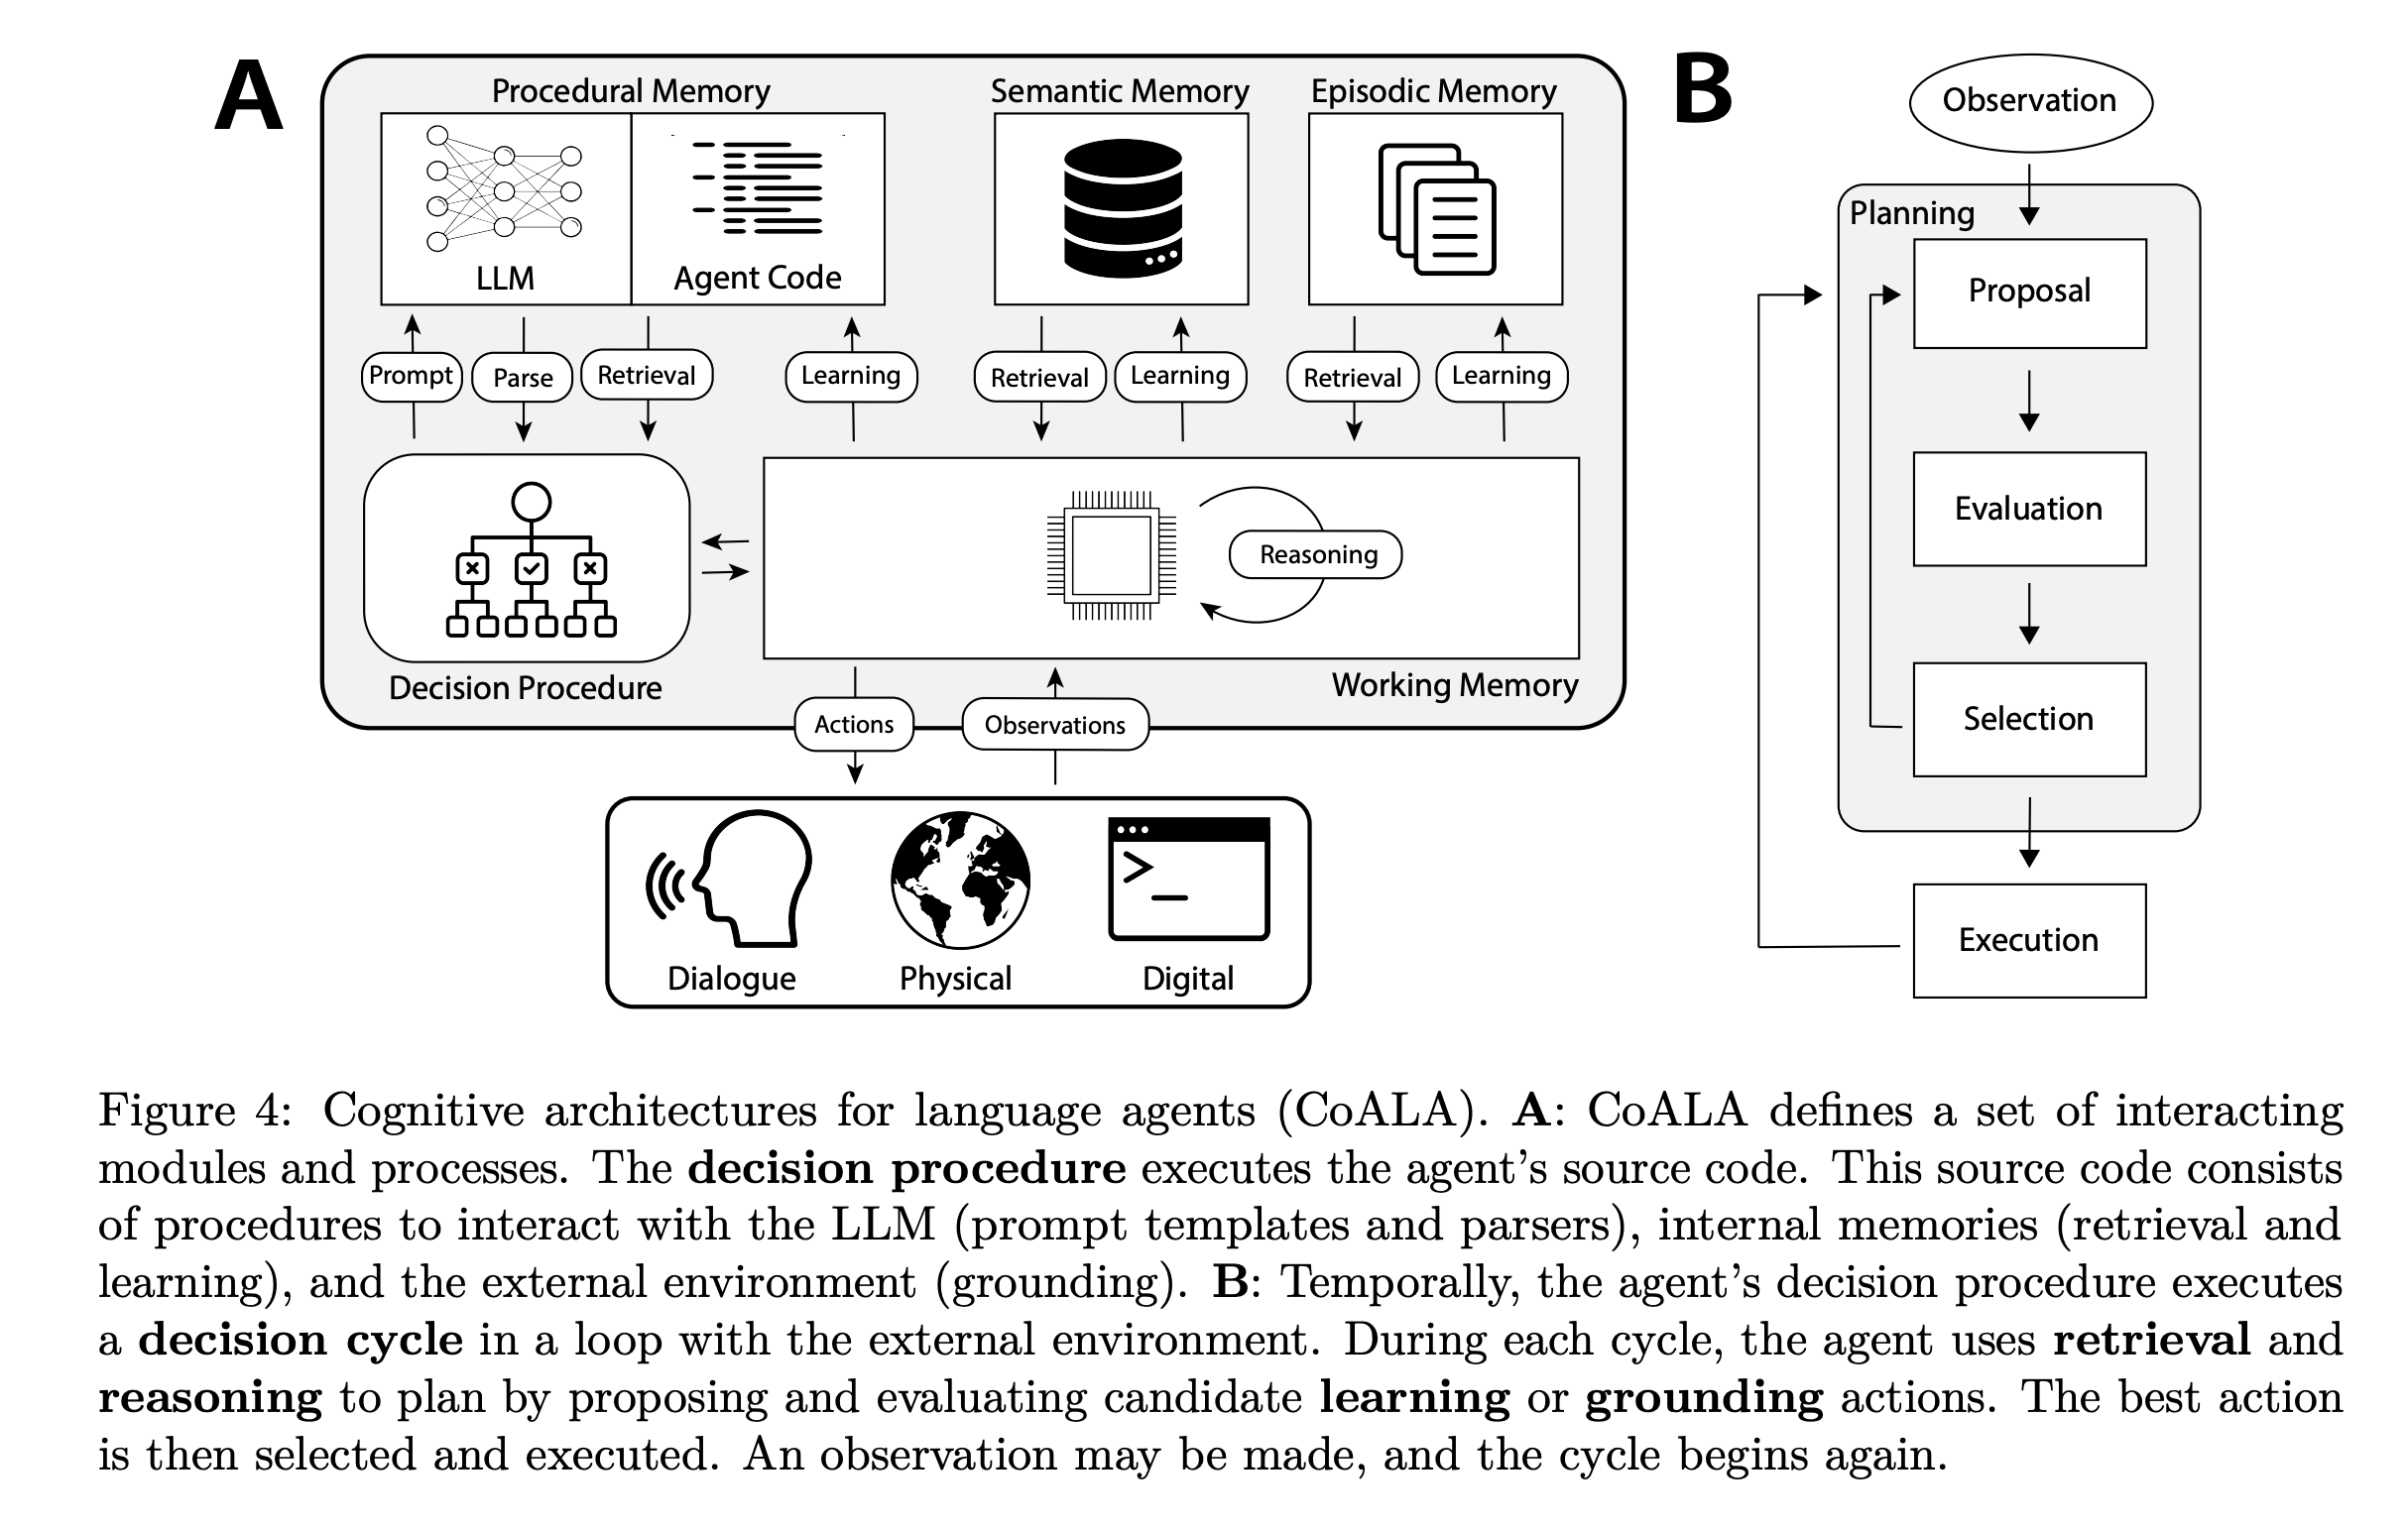
\includegraphics[width=0.85\linewidth]{assets/three-types-of-memory.png}
\end{center}

\textbf{三类记忆与 Skills 的定位}

认知科学将长期记忆大致分为三类：情景记忆（episodic memory，发生过什么）、语义记忆（semantic memory，知道什么）、程序性记忆（procedural memory，会做什么）。Agent 记忆的研究沿用了这套分类，\weblink{https://arxiv.org/abs/2309.02427}{CoALA} 按此三类组织 Agent 的长期记忆，并将程序性记忆进一步区分为两种形态：隐式的，存在模型权重中；显式的，写在 Agent 的代码或结构化的 Context 中。

沿用这一框架，Skills 可以理解为显式程序性记忆的一种标准化载体。引言中的命名考据在此形成呼应：Anthropic 选择 “Procedural” 一词，实际上从起点就将 Skills 定位在程序性记忆的范畴内。CoALA 内还提到一个结论：\textbf{向程序性记忆写入，比写入情景或语义记忆的风险更高，更容易引入 bug 或偏离设计意图}。这一结论与 Appendix D 的实验数据相互印证。

\textbf{从情景记忆到两种学习范式}

对应到 Agent 系统中，情景记忆的原始形态就是 Session 轨迹。但没有人会直接将原始 Session 当作记忆系统使用：信息密度低、噪声高，每次复用都需要重新读取全文。它真正的角色是\textbf{原料}：语义记忆和程序性记忆，是从这份原料中提炼出的两种产物，分别对应两条不同的路线。

\textbf{路线一：全自动提取。}Claude Code 的 auto-memory 在后台 fork 一个 Subagent，按阈值设置（默认每轮对话后）周期性提取对话要点；产物是四类记忆文件，内容偏向\textbf{信息性上下文}。加载环节我在 2.4 节具体提过，这里不是重点（机制图也见 2.4 节）。

\textbf{路线二：Human-in-the-loop 沉淀。}即 3.2 节中的 \code{contexts/} 工作流。人参与筛选哪些经验值得固化，产物是程序性知识，最终落入 Context 文件或 Skill。

\textbf{取舍与展望}

目前我的判断是：全自动路线降低了维护成本，但学习的东西缺乏人工把关，质量存在波动（方向偏离），这是我将 \code{autoMemoryEnabled} 关闭的原因；Human-in-the-loop 的维护成本更高，但每条记忆都经过人的判断与筛选，SkillsBench 的实验（Appendix D）也更倾向于支持这一方向。

往后看，两条路线未必始终对立。自动提取、人工批准的中间形态，也许是更可持续的方向。这里记录的只是 2026 年年中的一个阶段性观察。

\opsectionx{Appendix D}{SkillsBench 的结论}

\weblink{https://www.oreilly.com/radar/agent-skills-work-but-the-research-shows-most-teams-are-building-them-wrong/}{SkillsBench} 的对照实验（84 个任务、11 个领域）提供了几项值得关注的结论。

\begin{center}
  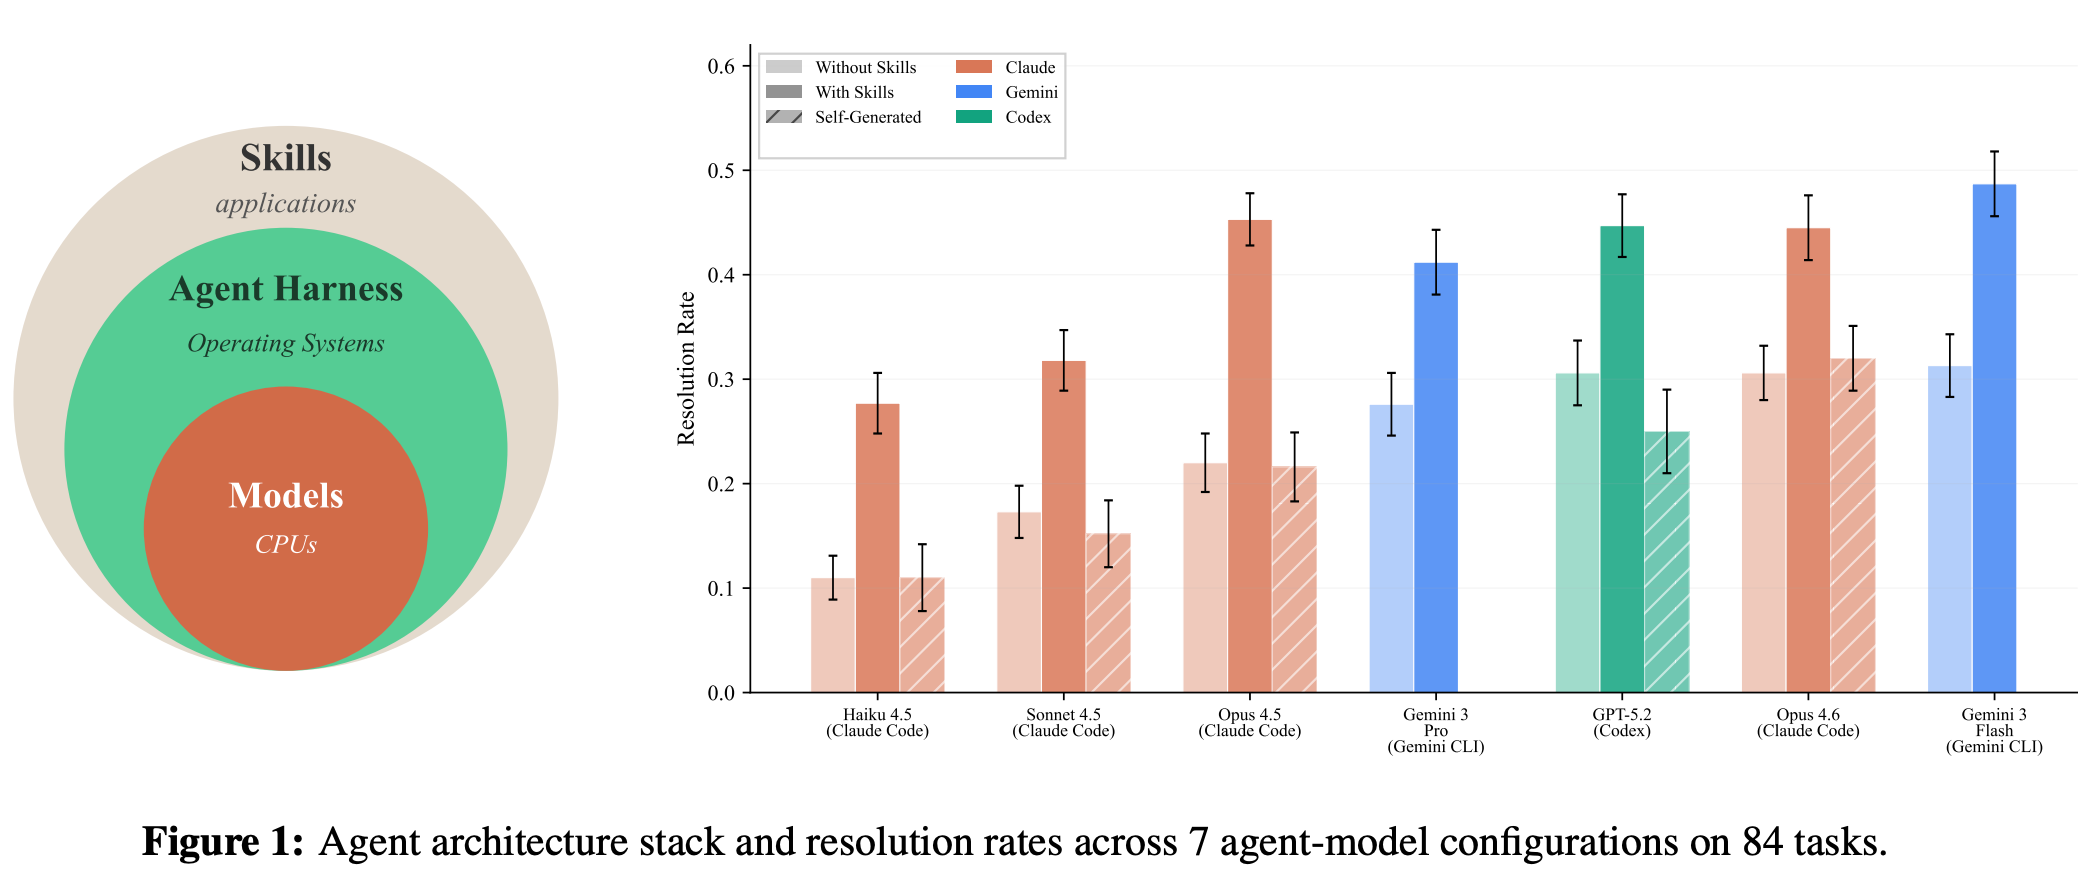
\includegraphics[width=0.92\linewidth]{assets/skillsbench-evaluation-results.png}
\end{center}

\begin{optable}
\begin{tabularx}{\linewidth}{@{}l>{\raggedright\arraybackslash}X@{}}
\toprule
\tabhead{发现} & \tabhead{含义} \\
\midrule
经人工筛选与精修的 Skill 平均提升 \textbf{16.2\%} & Skill 有用，但\textbf{前提是由人来把关质量} \\
Healthcare 提升 ${\sim}52\%$，SWE 仅 4.5\% & 模型预训练覆盖越薄弱的领域，Skill 的边际收益越大 \\
模型自生成的 Skill 提升 \textbf{0\%} & 让模型自己编写 Skill 再自己执行，没有正收益 \\
小模型 + 精修 Skill $\approx$ 大模型裸跑 & Skill 是一种\textbf{变相的模型能力升级} \\
\bottomrule
\end{tabularx}
\end{optable}

第三行最值得关注。让 Agent 自己编写 Skill，听上去已经接近自我迭代，但实验给出的答案是没有收益。背后的逻辑我认为是：Skill 本质上是对已有知识的程序化封装，而模型在缺乏外部可验证信号时无法从\textbf{自己身上蒸馏出自己尚未掌握的知识}，正如 RLHF 之所以需要 Human，正是因为模型无法可靠地充当自己的裁判。\textbf{在持续学习这条路径上，至少在质量把关这一环，短期内仍然离不开人的判断。}

这也解释了 3.2 节中 \code{contexts/} 工作流为何必须由人来收尾：将预测结果与标准答案进行对比，这件事可以交给 Agent 执行；但\textbf{哪些结论值得更新到 Context 中的判断，仍需由人来决策}。


\end{document}
